\documentclass[twoside]{book}

% Packages required by doxygen
\usepackage{fixltx2e}
\usepackage{calc}
\usepackage{doxygen}
\usepackage[export]{adjustbox} % also loads graphicx
\usepackage{graphicx}
\usepackage[utf8]{inputenc}
\usepackage{makeidx}
\usepackage{multicol}
\usepackage{multirow}
\PassOptionsToPackage{warn}{textcomp}
\usepackage{textcomp}
\usepackage[nointegrals]{wasysym}
\usepackage[table]{xcolor}

% Font selection
\usepackage[T1]{fontenc}
\usepackage[scaled=.90]{helvet}
\usepackage{courier}
\usepackage{amssymb}
\usepackage{sectsty}
\renewcommand{\familydefault}{\sfdefault}
\allsectionsfont{%
  \fontseries{bc}\selectfont%
  \color{darkgray}%
}
\renewcommand{\DoxyLabelFont}{%
  \fontseries{bc}\selectfont%
  \color{darkgray}%
}
\newcommand{\+}{\discretionary{\mbox{\scriptsize$\hookleftarrow$}}{}{}}

% Page & text layout
\usepackage{geometry}
\geometry{%
  a4paper,%
  top=2.5cm,%
  bottom=2.5cm,%
  left=2.5cm,%
  right=2.5cm%
}
\tolerance=750
\hfuzz=15pt
\hbadness=750
\setlength{\emergencystretch}{15pt}
\setlength{\parindent}{0cm}
\setlength{\parskip}{3ex plus 2ex minus 2ex}
\makeatletter
\renewcommand{\paragraph}{%
  \@startsection{paragraph}{4}{0ex}{-1.0ex}{1.0ex}{%
    \normalfont\normalsize\bfseries\SS@parafont%
  }%
}
\renewcommand{\subparagraph}{%
  \@startsection{subparagraph}{5}{0ex}{-1.0ex}{1.0ex}{%
    \normalfont\normalsize\bfseries\SS@subparafont%
  }%
}
\makeatother

% Headers & footers
\usepackage{fancyhdr}
\pagestyle{fancyplain}
\fancyhead[LE]{\fancyplain{}{\bfseries\thepage}}
\fancyhead[CE]{\fancyplain{}{}}
\fancyhead[RE]{\fancyplain{}{\bfseries\leftmark}}
\fancyhead[LO]{\fancyplain{}{\bfseries\rightmark}}
\fancyhead[CO]{\fancyplain{}{}}
\fancyhead[RO]{\fancyplain{}{\bfseries\thepage}}
\fancyfoot[LE]{\fancyplain{}{}}
\fancyfoot[CE]{\fancyplain{}{}}
\fancyfoot[RE]{\fancyplain{}{\bfseries\scriptsize Generated by Doxygen }}
\fancyfoot[LO]{\fancyplain{}{\bfseries\scriptsize Generated by Doxygen }}
\fancyfoot[CO]{\fancyplain{}{}}
\fancyfoot[RO]{\fancyplain{}{}}
\renewcommand{\footrulewidth}{0.4pt}
\renewcommand{\chaptermark}[1]{%
  \markboth{#1}{}%
}
\renewcommand{\sectionmark}[1]{%
  \markright{\thesection\ #1}%
}

% Indices & bibliography
\usepackage{natbib}
\usepackage[titles]{tocloft}
\setcounter{tocdepth}{3}
\setcounter{secnumdepth}{5}
\makeindex

% Hyperlinks (required, but should be loaded last)
\usepackage{ifpdf}
\ifpdf
  \usepackage[pdftex,pagebackref=true]{hyperref}
\else
  \usepackage[ps2pdf,pagebackref=true]{hyperref}
\fi
\hypersetup{%
  colorlinks=true,%
  linkcolor=blue,%
  citecolor=blue,%
  unicode%
}

% Custom commands
\newcommand{\clearemptydoublepage}{%
  \newpage{\pagestyle{empty}\cleardoublepage}%
}

\usepackage{caption}
\captionsetup{labelsep=space,justification=centering,font={bf},singlelinecheck=off,skip=4pt,position=top}

%===== C O N T E N T S =====

\begin{document}

% Titlepage & ToC
\hypersetup{pageanchor=false,
             bookmarksnumbered=true,
             pdfencoding=unicode
            }
\pagenumbering{alph}
\begin{titlepage}
\vspace*{7cm}
\begin{center}%
{\Large Stompy Blondie Unity Tools }\\
\vspace*{1cm}
{\large Generated by Doxygen 1.8.14}\\
\end{center}
\end{titlepage}
\clearemptydoublepage
\pagenumbering{roman}
\tableofcontents
\clearemptydoublepage
\pagenumbering{arabic}
\hypersetup{pageanchor=true}

%--- Begin generated contents ---
\chapter{Stompy Blondie Unity Tools}
\label{md__r_e_a_d_m_e}
\Hypertarget{md__r_e_a_d_m_e}
This is a bunch of utility classes and other stuff that can be used by anyone in their Unity3D projects. Or for reference, you know.

Most of the classes have at least some semblance of documentation in them.

\subsection*{Classes }

{\bfseries To be filled}

\subsection*{Requires }


\begin{DoxyItemize}
\item Json.\+N\+ET
\end{DoxyItemize}

\subsection*{Installation }

Check out the repository in your scripts directory. You will to add any code that uses any of the classes to an assembly definition so you can reference the Stompy\+Blondie\+Unity\+Tools assembly.

\subsection*{License }

It\textquotesingle{}s M\+IT, do what you like with it.

\subsection*{Contact }

Fiona -\/ \href{mailto:yum@fiona.pizza}{\tt yum@fiona.\+pizza} 
\chapter{Namespace Index}
\section{Namespace List}
Here is a list of all namespaces with brief descriptions\+:\begin{DoxyCompactList}
\item\contentsline{section}{\mbox{\hyperlink{namespace_stompy_blondie}{Stompy\+Blondie}} }{\pageref{namespace_stompy_blondie}}{}
\item\contentsline{section}{\mbox{\hyperlink{namespace_stompy_blondie_1_1_a_i}{Stompy\+Blondie.\+AI}} }{\pageref{namespace_stompy_blondie_1_1_a_i}}{}
\item\contentsline{section}{\mbox{\hyperlink{namespace_stompy_blondie_1_1_behaviours}{Stompy\+Blondie.\+Behaviours}} }{\pageref{namespace_stompy_blondie_1_1_behaviours}}{}
\item\contentsline{section}{\mbox{\hyperlink{namespace_stompy_blondie_1_1_common}{Stompy\+Blondie.\+Common}} }{\pageref{namespace_stompy_blondie_1_1_common}}{}
\item\contentsline{section}{\mbox{\hyperlink{namespace_stompy_blondie_1_1_common_1_1_types}{Stompy\+Blondie.\+Common.\+Types}} }{\pageref{namespace_stompy_blondie_1_1_common_1_1_types}}{}
\item\contentsline{section}{\mbox{\hyperlink{namespace_stompy_blondie_1_1_extensions}{Stompy\+Blondie.\+Extensions}} }{\pageref{namespace_stompy_blondie_1_1_extensions}}{}
\item\contentsline{section}{\mbox{\hyperlink{namespace_stompy_blondie_1_1_math}{Stompy\+Blondie.\+Math}} }{\pageref{namespace_stompy_blondie_1_1_math}}{}
\item\contentsline{section}{\mbox{\hyperlink{namespace_stompy_blondie_1_1_systems}{Stompy\+Blondie.\+Systems}} }{\pageref{namespace_stompy_blondie_1_1_systems}}{}
\item\contentsline{section}{\mbox{\hyperlink{namespace_stompy_blondie_1_1_tests}{Stompy\+Blondie.\+Tests}} }{\pageref{namespace_stompy_blondie_1_1_tests}}{}
\item\contentsline{section}{\mbox{\hyperlink{namespace_stompy_blondie_1_1_utils}{Stompy\+Blondie.\+Utils}} }{\pageref{namespace_stompy_blondie_1_1_utils}}{}
\end{DoxyCompactList}

\chapter{Hierarchical Index}
\section{Class Hierarchy}
This inheritance list is sorted roughly, but not completely, alphabetically\+:\begin{DoxyCompactList}
\item \contentsline{section}{Stompy\+Blondie.\+Math.\+A\+Star}{\pageref{class_stompy_blondie_1_1_math_1_1_a_star}}{}
\item \contentsline{section}{Stompy\+Blondie.\+Math.\+A\+Star\+Node}{\pageref{class_stompy_blondie_1_1_math_1_1_a_star_node}}{}
\item \contentsline{section}{Stompy\+Blondie.\+Tests.\+A\+Star\+Test}{\pageref{class_stompy_blondie_1_1_tests_1_1_a_star_test}}{}
\item \contentsline{section}{Stompy\+Blondie.\+Systems.\+Effect}{\pageref{class_stompy_blondie_1_1_systems_1_1_effect}}{}
\item I\+Enumerable\begin{DoxyCompactList}
\item \contentsline{section}{Stompy\+Blondie.\+Utils.\+Time\+Lerper}{\pageref{class_stompy_blondie_1_1_utils_1_1_time_lerper}}{}
\end{DoxyCompactList}
\item I\+Enumerator\begin{DoxyCompactList}
\item \contentsline{section}{Stompy\+Blondie.\+Utils.\+Time\+Lerp}{\pageref{class_stompy_blondie_1_1_utils_1_1_time_lerp}}{}
\end{DoxyCompactList}
\item I\+Pointer\+Enter\+Handler\begin{DoxyCompactList}
\item \contentsline{section}{Stompy\+Blondie.\+Behaviours.\+Is\+Mouse\+Over}{\pageref{class_stompy_blondie_1_1_behaviours_1_1_is_mouse_over}}{}
\end{DoxyCompactList}
\item I\+Pointer\+Exit\+Handler\begin{DoxyCompactList}
\item \contentsline{section}{Stompy\+Blondie.\+Behaviours.\+Is\+Mouse\+Over}{\pageref{class_stompy_blondie_1_1_behaviours_1_1_is_mouse_over}}{}
\end{DoxyCompactList}
\item Mono\+Behaviour\begin{DoxyCompactList}
\item \contentsline{section}{Stompy\+Blondie.\+A\+I.\+Navigation\+Map\+Debug\+Renderer}{\pageref{class_stompy_blondie_1_1_a_i_1_1_navigation_map_debug_renderer}}{}
\item \contentsline{section}{Stompy\+Blondie.\+Behaviours.\+Bobber}{\pageref{class_stompy_blondie_1_1_behaviours_1_1_bobber}}{}
\item \contentsline{section}{Stompy\+Blondie.\+Behaviours.\+Face\+Camera}{\pageref{class_stompy_blondie_1_1_behaviours_1_1_face_camera}}{}
\item \contentsline{section}{Stompy\+Blondie.\+Behaviours.\+Is\+Mouse\+Over}{\pageref{class_stompy_blondie_1_1_behaviours_1_1_is_mouse_over}}{}
\item \contentsline{section}{Stompy\+Blondie.\+Behaviours.\+Spinner}{\pageref{class_stompy_blondie_1_1_behaviours_1_1_spinner}}{}
\item \contentsline{section}{Stompy\+Blondie.\+Extensions.\+Extension\+Mono\+Behaviour}{\pageref{class_stompy_blondie_1_1_extensions_1_1_extension_mono_behaviour}}{}
\item \contentsline{section}{Stompy\+Blondie.\+Systems.\+Effects\+Manager}{\pageref{class_stompy_blondie_1_1_systems_1_1_effects_manager}}{}
\item \contentsline{section}{Stompy\+Blondie.\+Utils.\+Bone\+Clone}{\pageref{class_stompy_blondie_1_1_utils_1_1_bone_clone}}{}
\end{DoxyCompactList}
\item \contentsline{section}{Stompy\+Blondie.\+A\+I.\+Navigation\+Map}{\pageref{class_stompy_blondie_1_1_a_i_1_1_navigation_map}}{}
\item \contentsline{section}{Stompy\+Blondie.\+A\+I.\+Navigation\+Point}{\pageref{struct_stompy_blondie_1_1_a_i_1_1_navigation_point}}{}
\item \contentsline{section}{Stompy\+Blondie.\+A\+I.\+Navigation\+Point\+Link}{\pageref{struct_stompy_blondie_1_1_a_i_1_1_navigation_point_link}}{}
\item \contentsline{section}{Stompy\+Blondie.\+Common.\+Types.\+Pos}{\pageref{struct_stompy_blondie_1_1_common_1_1_types_1_1_pos}}{}
\item \contentsline{section}{Stompy\+Blondie.\+Common.\+Ref$<$ T $>$}{\pageref{class_stompy_blondie_1_1_common_1_1_ref}}{}
\item \contentsline{section}{Stompy\+Blondie.\+A\+I.\+Tilemap\+Navigation}{\pageref{class_stompy_blondie_1_1_a_i_1_1_tilemap_navigation}}{}
\end{DoxyCompactList}

\chapter{Class Index}
\section{Class List}
Here are the classes, structs, unions and interfaces with brief descriptions\+:\begin{DoxyCompactList}
\item\contentsline{section}{\mbox{\hyperlink{class_stompy_blondie_1_1_math_1_1_a_star}{Stompy\+Blondie.\+Math.\+A\+Star}} }{\pageref{class_stompy_blondie_1_1_math_1_1_a_star}}{}
\item\contentsline{section}{\mbox{\hyperlink{class_stompy_blondie_1_1_math_1_1_a_star_node}{Stompy\+Blondie.\+Math.\+A\+Star\+Node}} }{\pageref{class_stompy_blondie_1_1_math_1_1_a_star_node}}{}
\item\contentsline{section}{\mbox{\hyperlink{class_stompy_blondie_1_1_tests_1_1_a_star_test}{Stompy\+Blondie.\+Tests.\+A\+Star\+Test}} }{\pageref{class_stompy_blondie_1_1_tests_1_1_a_star_test}}{}
\item\contentsline{section}{\mbox{\hyperlink{class_stompy_blondie_1_1_behaviours_1_1_bobber}{Stompy\+Blondie.\+Behaviours.\+Bobber}} }{\pageref{class_stompy_blondie_1_1_behaviours_1_1_bobber}}{}
\item\contentsline{section}{\mbox{\hyperlink{class_stompy_blondie_1_1_utils_1_1_bone_clone}{Stompy\+Blondie.\+Utils.\+Bone\+Clone}} }{\pageref{class_stompy_blondie_1_1_utils_1_1_bone_clone}}{}
\item\contentsline{section}{\mbox{\hyperlink{class_stompy_blondie_1_1_systems_1_1_effect}{Stompy\+Blondie.\+Systems.\+Effect}} }{\pageref{class_stompy_blondie_1_1_systems_1_1_effect}}{}
\item\contentsline{section}{\mbox{\hyperlink{class_stompy_blondie_1_1_systems_1_1_effects_manager}{Stompy\+Blondie.\+Systems.\+Effects\+Manager}} }{\pageref{class_stompy_blondie_1_1_systems_1_1_effects_manager}}{}
\item\contentsline{section}{\mbox{\hyperlink{class_stompy_blondie_1_1_extensions_1_1_extension_mono_behaviour}{Stompy\+Blondie.\+Extensions.\+Extension\+Mono\+Behaviour}} }{\pageref{class_stompy_blondie_1_1_extensions_1_1_extension_mono_behaviour}}{}
\item\contentsline{section}{\mbox{\hyperlink{class_stompy_blondie_1_1_behaviours_1_1_face_camera}{Stompy\+Blondie.\+Behaviours.\+Face\+Camera}} }{\pageref{class_stompy_blondie_1_1_behaviours_1_1_face_camera}}{}
\item\contentsline{section}{\mbox{\hyperlink{class_stompy_blondie_1_1_behaviours_1_1_is_mouse_over}{Stompy\+Blondie.\+Behaviours.\+Is\+Mouse\+Over}} }{\pageref{class_stompy_blondie_1_1_behaviours_1_1_is_mouse_over}}{}
\item\contentsline{section}{\mbox{\hyperlink{class_stompy_blondie_1_1_a_i_1_1_navigation_map}{Stompy\+Blondie.\+A\+I.\+Navigation\+Map}} }{\pageref{class_stompy_blondie_1_1_a_i_1_1_navigation_map}}{}
\item\contentsline{section}{\mbox{\hyperlink{class_stompy_blondie_1_1_a_i_1_1_navigation_map_debug_renderer}{Stompy\+Blondie.\+A\+I.\+Navigation\+Map\+Debug\+Renderer}} }{\pageref{class_stompy_blondie_1_1_a_i_1_1_navigation_map_debug_renderer}}{}
\item\contentsline{section}{\mbox{\hyperlink{struct_stompy_blondie_1_1_a_i_1_1_navigation_point}{Stompy\+Blondie.\+A\+I.\+Navigation\+Point}} }{\pageref{struct_stompy_blondie_1_1_a_i_1_1_navigation_point}}{}
\item\contentsline{section}{\mbox{\hyperlink{struct_stompy_blondie_1_1_a_i_1_1_navigation_point_link}{Stompy\+Blondie.\+A\+I.\+Navigation\+Point\+Link}} }{\pageref{struct_stompy_blondie_1_1_a_i_1_1_navigation_point_link}}{}
\item\contentsline{section}{\mbox{\hyperlink{struct_stompy_blondie_1_1_common_1_1_types_1_1_pos}{Stompy\+Blondie.\+Common.\+Types.\+Pos}} }{\pageref{struct_stompy_blondie_1_1_common_1_1_types_1_1_pos}}{}
\item\contentsline{section}{\mbox{\hyperlink{class_stompy_blondie_1_1_common_1_1_ref}{Stompy\+Blondie.\+Common.\+Ref$<$ T $>$}} }{\pageref{class_stompy_blondie_1_1_common_1_1_ref}}{}
\item\contentsline{section}{\mbox{\hyperlink{class_stompy_blondie_1_1_behaviours_1_1_spinner}{Stompy\+Blondie.\+Behaviours.\+Spinner}} }{\pageref{class_stompy_blondie_1_1_behaviours_1_1_spinner}}{}
\item\contentsline{section}{\mbox{\hyperlink{class_stompy_blondie_1_1_a_i_1_1_tilemap_navigation}{Stompy\+Blondie.\+A\+I.\+Tilemap\+Navigation}} }{\pageref{class_stompy_blondie_1_1_a_i_1_1_tilemap_navigation}}{}
\item\contentsline{section}{\mbox{\hyperlink{class_stompy_blondie_1_1_utils_1_1_time_lerp}{Stompy\+Blondie.\+Utils.\+Time\+Lerp}} }{\pageref{class_stompy_blondie_1_1_utils_1_1_time_lerp}}{}
\item\contentsline{section}{\mbox{\hyperlink{class_stompy_blondie_1_1_utils_1_1_time_lerper}{Stompy\+Blondie.\+Utils.\+Time\+Lerper}} }{\pageref{class_stompy_blondie_1_1_utils_1_1_time_lerper}}{}
\end{DoxyCompactList}

\chapter{File Index}
\section{File List}
Here is a list of all files with brief descriptions\+:\begin{DoxyCompactList}
\item\contentsline{section}{A\+I/\mbox{\hyperlink{_navigation_map_debug_renderer_8cs}{Navigation\+Map\+Debug\+Renderer.\+cs}} }{\pageref{_navigation_map_debug_renderer_8cs}}{}
\item\contentsline{section}{A\+I/\mbox{\hyperlink{_tilemap_navigation_8cs}{Tilemap\+Navigation.\+cs}} }{\pageref{_tilemap_navigation_8cs}}{}
\item\contentsline{section}{Behaviours/\mbox{\hyperlink{_bobber_8cs}{Bobber.\+cs}} }{\pageref{_bobber_8cs}}{}
\item\contentsline{section}{Behaviours/\mbox{\hyperlink{_face_camera_8cs}{Face\+Camera.\+cs}} }{\pageref{_face_camera_8cs}}{}
\item\contentsline{section}{Behaviours/\mbox{\hyperlink{_is_mouse_over_8cs}{Is\+Mouse\+Over.\+cs}} }{\pageref{_is_mouse_over_8cs}}{}
\item\contentsline{section}{Behaviours/\mbox{\hyperlink{_spinner_8cs}{Spinner.\+cs}} }{\pageref{_spinner_8cs}}{}
\item\contentsline{section}{Common/\mbox{\hyperlink{_ref_8cs}{Ref.\+cs}} }{\pageref{_ref_8cs}}{}
\item\contentsline{section}{Common/\mbox{\hyperlink{_types_8cs}{Types.\+cs}} }{\pageref{_types_8cs}}{}
\item\contentsline{section}{Editor/\mbox{\hyperlink{_scene_auto_loader_8cs}{Scene\+Auto\+Loader.\+cs}} }{\pageref{_scene_auto_loader_8cs}}{}
\item\contentsline{section}{Extensions/\mbox{\hyperlink{_extension_audio_source_8cs}{Extension\+Audio\+Source.\+cs}} }{\pageref{_extension_audio_source_8cs}}{}
\item\contentsline{section}{Extensions/\mbox{\hyperlink{_extension_mono_behaviour_8cs}{Extension\+Mono\+Behaviour.\+cs}} }{\pageref{_extension_mono_behaviour_8cs}}{}
\item\contentsline{section}{Extensions/\mbox{\hyperlink{_extension_unity_vector3_8cs}{Extension\+Unity\+Vector3.\+cs}} }{\pageref{_extension_unity_vector3_8cs}}{}
\item\contentsline{section}{Math/\mbox{\hyperlink{_a_star_8cs}{A\+Star.\+cs}} }{\pageref{_a_star_8cs}}{}
\item\contentsline{section}{Systems/\mbox{\hyperlink{_effects_manager_8cs}{Effects\+Manager.\+cs}} }{\pageref{_effects_manager_8cs}}{}
\item\contentsline{section}{Tests/\mbox{\hyperlink{_a_star_8spec_8cs}{A\+Star.\+spec.\+cs}} }{\pageref{_a_star_8spec_8cs}}{}
\item\contentsline{section}{Utils/\mbox{\hyperlink{_bone_clone_8cs}{Bone\+Clone.\+cs}} }{\pageref{_bone_clone_8cs}}{}
\item\contentsline{section}{Utils/\mbox{\hyperlink{_direction_helper_8cs}{Direction\+Helper.\+cs}} }{\pageref{_direction_helper_8cs}}{}
\item\contentsline{section}{Utils/\mbox{\hyperlink{_extension_transform_8cs}{Extension\+Transform.\+cs}} }{\pageref{_extension_transform_8cs}}{}
\item\contentsline{section}{Utils/\mbox{\hyperlink{_lerp_helper_8cs}{Lerp\+Helper.\+cs}} }{\pageref{_lerp_helper_8cs}}{}
\item\contentsline{section}{Utils/\mbox{\hyperlink{_scrollbar_helper_8cs}{Scrollbar\+Helper.\+cs}} }{\pageref{_scrollbar_helper_8cs}}{}
\end{DoxyCompactList}

\chapter{Namespace Documentation}
\hypertarget{namespace_stompy_blondie}{}\section{Stompy\+Blondie Namespace Reference}
\label{namespace_stompy_blondie}\index{Stompy\+Blondie@{Stompy\+Blondie}}
\subsection*{Namespaces}
\begin{DoxyCompactItemize}
\end{DoxyCompactItemize}

\hypertarget{namespace_stompy_blondie_1_1_a_i}{}\section{Stompy\+Blondie.\+AI Namespace Reference}
\label{namespace_stompy_blondie_1_1_a_i}\index{Stompy\+Blondie.\+AI@{Stompy\+Blondie.\+AI}}
\subsection*{Classes}
\begin{DoxyCompactItemize}
\item 
class \mbox{\hyperlink{class_stompy_blondie_1_1_a_i_1_1_navigation_map}{Navigation\+Map}}
\item 
class \mbox{\hyperlink{class_stompy_blondie_1_1_a_i_1_1_navigation_map_debug_renderer}{Navigation\+Map\+Debug\+Renderer}}
\item 
struct \mbox{\hyperlink{struct_stompy_blondie_1_1_a_i_1_1_navigation_point}{Navigation\+Point}}
\item 
struct \mbox{\hyperlink{struct_stompy_blondie_1_1_a_i_1_1_navigation_point_link}{Navigation\+Point\+Link}}
\item 
class \mbox{\hyperlink{class_stompy_blondie_1_1_a_i_1_1_tilemap_navigation}{Tilemap\+Navigation}}
\end{DoxyCompactItemize}

\hypertarget{namespace_stompy_blondie_1_1_behaviours}{}\section{Stompy\+Blondie.\+Behaviours Namespace Reference}
\label{namespace_stompy_blondie_1_1_behaviours}\index{Stompy\+Blondie.\+Behaviours@{Stompy\+Blondie.\+Behaviours}}
\subsection*{Classes}
\begin{DoxyCompactItemize}
\item 
class \mbox{\hyperlink{class_stompy_blondie_1_1_behaviours_1_1_bobber}{Bobber}}
\item 
class \mbox{\hyperlink{class_stompy_blondie_1_1_behaviours_1_1_face_camera}{Face\+Camera}}
\item 
class \mbox{\hyperlink{class_stompy_blondie_1_1_behaviours_1_1_is_mouse_over}{Is\+Mouse\+Over}}
\item 
class \mbox{\hyperlink{class_stompy_blondie_1_1_behaviours_1_1_spinner}{Spinner}}
\end{DoxyCompactItemize}

\hypertarget{namespace_stompy_blondie_1_1_common}{}\section{Stompy\+Blondie.\+Common Namespace Reference}
\label{namespace_stompy_blondie_1_1_common}\index{Stompy\+Blondie.\+Common@{Stompy\+Blondie.\+Common}}
\subsection*{Namespaces}
\begin{DoxyCompactItemize}
\item 
namespace \mbox{\hyperlink{namespace_stompy_blondie_1_1_common_1_1_types}{Types}}
\end{DoxyCompactItemize}
\subsection*{Classes}
\begin{DoxyCompactItemize}
\item 
class \mbox{\hyperlink{class_stompy_blondie_1_1_common_1_1_ref}{Ref}}
\end{DoxyCompactItemize}

\hypertarget{namespace_stompy_blondie_1_1_common_1_1_types}{}\section{Stompy\+Blondie.\+Common.\+Types Namespace Reference}
\label{namespace_stompy_blondie_1_1_common_1_1_types}\index{Stompy\+Blondie.\+Common.\+Types@{Stompy\+Blondie.\+Common.\+Types}}
\subsection*{Classes}
\begin{DoxyCompactItemize}
\item 
struct \mbox{\hyperlink{struct_stompy_blondie_1_1_common_1_1_types_1_1_pos}{Pos}}
\item 
class {\bfseries Pos\+Type\+Converter}
\end{DoxyCompactItemize}
\subsection*{Enumerations}
\begin{DoxyCompactItemize}
\item 
enum \mbox{\hyperlink{namespace_stompy_blondie_1_1_common_1_1_types_a2477d455b973b989d248635a56ffbd25}{Direction}} \{ \mbox{\hyperlink{namespace_stompy_blondie_1_1_common_1_1_types_a2477d455b973b989d248635a56ffbd25a08a38277b0309070706f6652eeae9a53}{Direction.\+Down}}, 
\mbox{\hyperlink{namespace_stompy_blondie_1_1_common_1_1_types_a2477d455b973b989d248635a56ffbd25a945d5e233cf7d6240f6b783b36a374ff}{Direction.\+Left}}, 
\mbox{\hyperlink{namespace_stompy_blondie_1_1_common_1_1_types_a2477d455b973b989d248635a56ffbd25a258f49887ef8d14ac268c92b02503aaa}{Direction.\+Up}}, 
\mbox{\hyperlink{namespace_stompy_blondie_1_1_common_1_1_types_a2477d455b973b989d248635a56ffbd25a92b09c7c48c520c3c55e497875da437c}{Direction.\+Right}}
 \}
\item 
enum \mbox{\hyperlink{namespace_stompy_blondie_1_1_common_1_1_types_a67d21ccf6a23cdea91c271cce76f920f}{Eight\+Direction}} \{ \newline
\mbox{\hyperlink{namespace_stompy_blondie_1_1_common_1_1_types_a67d21ccf6a23cdea91c271cce76f920fa08a38277b0309070706f6652eeae9a53}{Eight\+Direction.\+Down}}, 
\mbox{\hyperlink{namespace_stompy_blondie_1_1_common_1_1_types_a67d21ccf6a23cdea91c271cce76f920facd7f4772075da1452f8cd3648265b2c1}{Eight\+Direction.\+Down\+Left}}, 
\mbox{\hyperlink{namespace_stompy_blondie_1_1_common_1_1_types_a67d21ccf6a23cdea91c271cce76f920fa945d5e233cf7d6240f6b783b36a374ff}{Eight\+Direction.\+Left}}, 
\mbox{\hyperlink{namespace_stompy_blondie_1_1_common_1_1_types_a67d21ccf6a23cdea91c271cce76f920fa105736deb2f54f03c011e5f053e08d00}{Eight\+Direction.\+Left\+Up}}, 
\newline
\mbox{\hyperlink{namespace_stompy_blondie_1_1_common_1_1_types_a67d21ccf6a23cdea91c271cce76f920fa258f49887ef8d14ac268c92b02503aaa}{Eight\+Direction.\+Up}}, 
\mbox{\hyperlink{namespace_stompy_blondie_1_1_common_1_1_types_a67d21ccf6a23cdea91c271cce76f920faee94ab0297ae02df64791255d0a3551e}{Eight\+Direction.\+Up\+Right}}, 
\mbox{\hyperlink{namespace_stompy_blondie_1_1_common_1_1_types_a67d21ccf6a23cdea91c271cce76f920fa92b09c7c48c520c3c55e497875da437c}{Eight\+Direction.\+Right}}, 
\mbox{\hyperlink{namespace_stompy_blondie_1_1_common_1_1_types_a67d21ccf6a23cdea91c271cce76f920fac7ff24224bc4b699e06c58a663ac618c}{Eight\+Direction.\+Right\+Down}}
 \}
\item 
enum \mbox{\hyperlink{namespace_stompy_blondie_1_1_common_1_1_types_aa8d41922aaa5f468ef8e2c8f8e083084}{Rotational\+Direction}} \{ \mbox{\hyperlink{namespace_stompy_blondie_1_1_common_1_1_types_aa8d41922aaa5f468ef8e2c8f8e083084aba360a794737bcc8657a5b6e870d7ba8}{Rotational\+Direction.\+Clockwise}}, 
\mbox{\hyperlink{namespace_stompy_blondie_1_1_common_1_1_types_aa8d41922aaa5f468ef8e2c8f8e083084a3ac558edd1e7ab76b05ea7e3eef91b54}{Rotational\+Direction.\+Anti\+Clockwise}}
 \}
\end{DoxyCompactItemize}


\subsection{Enumeration Type Documentation}
\mbox{\Hypertarget{namespace_stompy_blondie_1_1_common_1_1_types_a2477d455b973b989d248635a56ffbd25}\label{namespace_stompy_blondie_1_1_common_1_1_types_a2477d455b973b989d248635a56ffbd25}} 
\index{Stompy\+Blondie\+::\+Common\+::\+Types@{Stompy\+Blondie\+::\+Common\+::\+Types}!Direction@{Direction}}
\index{Direction@{Direction}!Stompy\+Blondie\+::\+Common\+::\+Types@{Stompy\+Blondie\+::\+Common\+::\+Types}}
\subsubsection{\texorpdfstring{Direction}{Direction}}
{\footnotesize\ttfamily enum \mbox{\hyperlink{namespace_stompy_blondie_1_1_common_1_1_types_a2477d455b973b989d248635a56ffbd25}{Stompy\+Blondie.\+Common.\+Types.\+Direction}}\hspace{0.3cm}{\ttfamily [strong]}}

\begin{DoxyEnumFields}{Enumerator}
\raisebox{\heightof{T}}[0pt][0pt]{\index{Down@{Down}!Stompy\+Blondie\+::\+Common\+::\+Types@{Stompy\+Blondie\+::\+Common\+::\+Types}}\index{Stompy\+Blondie\+::\+Common\+::\+Types@{Stompy\+Blondie\+::\+Common\+::\+Types}!Down@{Down}}}\mbox{\Hypertarget{namespace_stompy_blondie_1_1_common_1_1_types_a2477d455b973b989d248635a56ffbd25a08a38277b0309070706f6652eeae9a53}\label{namespace_stompy_blondie_1_1_common_1_1_types_a2477d455b973b989d248635a56ffbd25a08a38277b0309070706f6652eeae9a53}} 
Down&\\
\hline

\raisebox{\heightof{T}}[0pt][0pt]{\index{Left@{Left}!Stompy\+Blondie\+::\+Common\+::\+Types@{Stompy\+Blondie\+::\+Common\+::\+Types}}\index{Stompy\+Blondie\+::\+Common\+::\+Types@{Stompy\+Blondie\+::\+Common\+::\+Types}!Left@{Left}}}\mbox{\Hypertarget{namespace_stompy_blondie_1_1_common_1_1_types_a2477d455b973b989d248635a56ffbd25a945d5e233cf7d6240f6b783b36a374ff}\label{namespace_stompy_blondie_1_1_common_1_1_types_a2477d455b973b989d248635a56ffbd25a945d5e233cf7d6240f6b783b36a374ff}} 
Left&\\
\hline

\raisebox{\heightof{T}}[0pt][0pt]{\index{Up@{Up}!Stompy\+Blondie\+::\+Common\+::\+Types@{Stompy\+Blondie\+::\+Common\+::\+Types}}\index{Stompy\+Blondie\+::\+Common\+::\+Types@{Stompy\+Blondie\+::\+Common\+::\+Types}!Up@{Up}}}\mbox{\Hypertarget{namespace_stompy_blondie_1_1_common_1_1_types_a2477d455b973b989d248635a56ffbd25a258f49887ef8d14ac268c92b02503aaa}\label{namespace_stompy_blondie_1_1_common_1_1_types_a2477d455b973b989d248635a56ffbd25a258f49887ef8d14ac268c92b02503aaa}} 
Up&\\
\hline

\raisebox{\heightof{T}}[0pt][0pt]{\index{Right@{Right}!Stompy\+Blondie\+::\+Common\+::\+Types@{Stompy\+Blondie\+::\+Common\+::\+Types}}\index{Stompy\+Blondie\+::\+Common\+::\+Types@{Stompy\+Blondie\+::\+Common\+::\+Types}!Right@{Right}}}\mbox{\Hypertarget{namespace_stompy_blondie_1_1_common_1_1_types_a2477d455b973b989d248635a56ffbd25a92b09c7c48c520c3c55e497875da437c}\label{namespace_stompy_blondie_1_1_common_1_1_types_a2477d455b973b989d248635a56ffbd25a92b09c7c48c520c3c55e497875da437c}} 
Right&\\
\hline

\end{DoxyEnumFields}
\mbox{\Hypertarget{namespace_stompy_blondie_1_1_common_1_1_types_a67d21ccf6a23cdea91c271cce76f920f}\label{namespace_stompy_blondie_1_1_common_1_1_types_a67d21ccf6a23cdea91c271cce76f920f}} 
\index{Stompy\+Blondie\+::\+Common\+::\+Types@{Stompy\+Blondie\+::\+Common\+::\+Types}!Eight\+Direction@{Eight\+Direction}}
\index{Eight\+Direction@{Eight\+Direction}!Stompy\+Blondie\+::\+Common\+::\+Types@{Stompy\+Blondie\+::\+Common\+::\+Types}}
\subsubsection{\texorpdfstring{Eight\+Direction}{EightDirection}}
{\footnotesize\ttfamily enum \mbox{\hyperlink{namespace_stompy_blondie_1_1_common_1_1_types_a67d21ccf6a23cdea91c271cce76f920f}{Stompy\+Blondie.\+Common.\+Types.\+Eight\+Direction}}\hspace{0.3cm}{\ttfamily [strong]}}

\begin{DoxyEnumFields}{Enumerator}
\raisebox{\heightof{T}}[0pt][0pt]{\index{Down@{Down}!Stompy\+Blondie\+::\+Common\+::\+Types@{Stompy\+Blondie\+::\+Common\+::\+Types}}\index{Stompy\+Blondie\+::\+Common\+::\+Types@{Stompy\+Blondie\+::\+Common\+::\+Types}!Down@{Down}}}\mbox{\Hypertarget{namespace_stompy_blondie_1_1_common_1_1_types_a67d21ccf6a23cdea91c271cce76f920fa08a38277b0309070706f6652eeae9a53}\label{namespace_stompy_blondie_1_1_common_1_1_types_a67d21ccf6a23cdea91c271cce76f920fa08a38277b0309070706f6652eeae9a53}} 
Down&\\
\hline

\raisebox{\heightof{T}}[0pt][0pt]{\index{Down\+Left@{Down\+Left}!Stompy\+Blondie\+::\+Common\+::\+Types@{Stompy\+Blondie\+::\+Common\+::\+Types}}\index{Stompy\+Blondie\+::\+Common\+::\+Types@{Stompy\+Blondie\+::\+Common\+::\+Types}!Down\+Left@{Down\+Left}}}\mbox{\Hypertarget{namespace_stompy_blondie_1_1_common_1_1_types_a67d21ccf6a23cdea91c271cce76f920facd7f4772075da1452f8cd3648265b2c1}\label{namespace_stompy_blondie_1_1_common_1_1_types_a67d21ccf6a23cdea91c271cce76f920facd7f4772075da1452f8cd3648265b2c1}} 
Down\+Left&\\
\hline

\raisebox{\heightof{T}}[0pt][0pt]{\index{Left@{Left}!Stompy\+Blondie\+::\+Common\+::\+Types@{Stompy\+Blondie\+::\+Common\+::\+Types}}\index{Stompy\+Blondie\+::\+Common\+::\+Types@{Stompy\+Blondie\+::\+Common\+::\+Types}!Left@{Left}}}\mbox{\Hypertarget{namespace_stompy_blondie_1_1_common_1_1_types_a67d21ccf6a23cdea91c271cce76f920fa945d5e233cf7d6240f6b783b36a374ff}\label{namespace_stompy_blondie_1_1_common_1_1_types_a67d21ccf6a23cdea91c271cce76f920fa945d5e233cf7d6240f6b783b36a374ff}} 
Left&\\
\hline

\raisebox{\heightof{T}}[0pt][0pt]{\index{Left\+Up@{Left\+Up}!Stompy\+Blondie\+::\+Common\+::\+Types@{Stompy\+Blondie\+::\+Common\+::\+Types}}\index{Stompy\+Blondie\+::\+Common\+::\+Types@{Stompy\+Blondie\+::\+Common\+::\+Types}!Left\+Up@{Left\+Up}}}\mbox{\Hypertarget{namespace_stompy_blondie_1_1_common_1_1_types_a67d21ccf6a23cdea91c271cce76f920fa105736deb2f54f03c011e5f053e08d00}\label{namespace_stompy_blondie_1_1_common_1_1_types_a67d21ccf6a23cdea91c271cce76f920fa105736deb2f54f03c011e5f053e08d00}} 
Left\+Up&\\
\hline

\raisebox{\heightof{T}}[0pt][0pt]{\index{Up@{Up}!Stompy\+Blondie\+::\+Common\+::\+Types@{Stompy\+Blondie\+::\+Common\+::\+Types}}\index{Stompy\+Blondie\+::\+Common\+::\+Types@{Stompy\+Blondie\+::\+Common\+::\+Types}!Up@{Up}}}\mbox{\Hypertarget{namespace_stompy_blondie_1_1_common_1_1_types_a67d21ccf6a23cdea91c271cce76f920fa258f49887ef8d14ac268c92b02503aaa}\label{namespace_stompy_blondie_1_1_common_1_1_types_a67d21ccf6a23cdea91c271cce76f920fa258f49887ef8d14ac268c92b02503aaa}} 
Up&\\
\hline

\raisebox{\heightof{T}}[0pt][0pt]{\index{Up\+Right@{Up\+Right}!Stompy\+Blondie\+::\+Common\+::\+Types@{Stompy\+Blondie\+::\+Common\+::\+Types}}\index{Stompy\+Blondie\+::\+Common\+::\+Types@{Stompy\+Blondie\+::\+Common\+::\+Types}!Up\+Right@{Up\+Right}}}\mbox{\Hypertarget{namespace_stompy_blondie_1_1_common_1_1_types_a67d21ccf6a23cdea91c271cce76f920faee94ab0297ae02df64791255d0a3551e}\label{namespace_stompy_blondie_1_1_common_1_1_types_a67d21ccf6a23cdea91c271cce76f920faee94ab0297ae02df64791255d0a3551e}} 
Up\+Right&\\
\hline

\raisebox{\heightof{T}}[0pt][0pt]{\index{Right@{Right}!Stompy\+Blondie\+::\+Common\+::\+Types@{Stompy\+Blondie\+::\+Common\+::\+Types}}\index{Stompy\+Blondie\+::\+Common\+::\+Types@{Stompy\+Blondie\+::\+Common\+::\+Types}!Right@{Right}}}\mbox{\Hypertarget{namespace_stompy_blondie_1_1_common_1_1_types_a67d21ccf6a23cdea91c271cce76f920fa92b09c7c48c520c3c55e497875da437c}\label{namespace_stompy_blondie_1_1_common_1_1_types_a67d21ccf6a23cdea91c271cce76f920fa92b09c7c48c520c3c55e497875da437c}} 
Right&\\
\hline

\raisebox{\heightof{T}}[0pt][0pt]{\index{Right\+Down@{Right\+Down}!Stompy\+Blondie\+::\+Common\+::\+Types@{Stompy\+Blondie\+::\+Common\+::\+Types}}\index{Stompy\+Blondie\+::\+Common\+::\+Types@{Stompy\+Blondie\+::\+Common\+::\+Types}!Right\+Down@{Right\+Down}}}\mbox{\Hypertarget{namespace_stompy_blondie_1_1_common_1_1_types_a67d21ccf6a23cdea91c271cce76f920fac7ff24224bc4b699e06c58a663ac618c}\label{namespace_stompy_blondie_1_1_common_1_1_types_a67d21ccf6a23cdea91c271cce76f920fac7ff24224bc4b699e06c58a663ac618c}} 
Right\+Down&\\
\hline

\end{DoxyEnumFields}
\mbox{\Hypertarget{namespace_stompy_blondie_1_1_common_1_1_types_aa8d41922aaa5f468ef8e2c8f8e083084}\label{namespace_stompy_blondie_1_1_common_1_1_types_aa8d41922aaa5f468ef8e2c8f8e083084}} 
\index{Stompy\+Blondie\+::\+Common\+::\+Types@{Stompy\+Blondie\+::\+Common\+::\+Types}!Rotational\+Direction@{Rotational\+Direction}}
\index{Rotational\+Direction@{Rotational\+Direction}!Stompy\+Blondie\+::\+Common\+::\+Types@{Stompy\+Blondie\+::\+Common\+::\+Types}}
\subsubsection{\texorpdfstring{Rotational\+Direction}{RotationalDirection}}
{\footnotesize\ttfamily enum \mbox{\hyperlink{namespace_stompy_blondie_1_1_common_1_1_types_aa8d41922aaa5f468ef8e2c8f8e083084}{Stompy\+Blondie.\+Common.\+Types.\+Rotational\+Direction}}\hspace{0.3cm}{\ttfamily [strong]}}

\begin{DoxyEnumFields}{Enumerator}
\raisebox{\heightof{T}}[0pt][0pt]{\index{Clockwise@{Clockwise}!Stompy\+Blondie\+::\+Common\+::\+Types@{Stompy\+Blondie\+::\+Common\+::\+Types}}\index{Stompy\+Blondie\+::\+Common\+::\+Types@{Stompy\+Blondie\+::\+Common\+::\+Types}!Clockwise@{Clockwise}}}\mbox{\Hypertarget{namespace_stompy_blondie_1_1_common_1_1_types_aa8d41922aaa5f468ef8e2c8f8e083084aba360a794737bcc8657a5b6e870d7ba8}\label{namespace_stompy_blondie_1_1_common_1_1_types_aa8d41922aaa5f468ef8e2c8f8e083084aba360a794737bcc8657a5b6e870d7ba8}} 
Clockwise&\\
\hline

\raisebox{\heightof{T}}[0pt][0pt]{\index{Anti\+Clockwise@{Anti\+Clockwise}!Stompy\+Blondie\+::\+Common\+::\+Types@{Stompy\+Blondie\+::\+Common\+::\+Types}}\index{Stompy\+Blondie\+::\+Common\+::\+Types@{Stompy\+Blondie\+::\+Common\+::\+Types}!Anti\+Clockwise@{Anti\+Clockwise}}}\mbox{\Hypertarget{namespace_stompy_blondie_1_1_common_1_1_types_aa8d41922aaa5f468ef8e2c8f8e083084a3ac558edd1e7ab76b05ea7e3eef91b54}\label{namespace_stompy_blondie_1_1_common_1_1_types_aa8d41922aaa5f468ef8e2c8f8e083084a3ac558edd1e7ab76b05ea7e3eef91b54}} 
Anti\+Clockwise&\\
\hline

\end{DoxyEnumFields}

\hypertarget{namespace_stompy_blondie_1_1_extensions}{}\section{Stompy\+Blondie.\+Extensions Namespace Reference}
\label{namespace_stompy_blondie_1_1_extensions}\index{Stompy\+Blondie.\+Extensions@{Stompy\+Blondie.\+Extensions}}
\subsection*{Classes}
\begin{DoxyCompactItemize}
\item 
class {\bfseries Extension\+Audio\+Source}
\item 
class \mbox{\hyperlink{class_stompy_blondie_1_1_extensions_1_1_extension_mono_behaviour}{Extension\+Mono\+Behaviour}}
\item 
class {\bfseries Extension\+Transform}
\item 
class {\bfseries Extension\+Unity\+Vector3}
\end{DoxyCompactItemize}

\hypertarget{namespace_stompy_blondie_1_1_math}{}\section{Stompy\+Blondie.\+Math Namespace Reference}
\label{namespace_stompy_blondie_1_1_math}\index{Stompy\+Blondie.\+Math@{Stompy\+Blondie.\+Math}}
\subsection*{Classes}
\begin{DoxyCompactItemize}
\item 
class \mbox{\hyperlink{class_stompy_blondie_1_1_math_1_1_a_star}{A\+Star}}
\item 
class \mbox{\hyperlink{class_stompy_blondie_1_1_math_1_1_a_star_node}{A\+Star\+Node}}
\end{DoxyCompactItemize}

\hypertarget{namespace_stompy_blondie_1_1_systems}{}\section{Stompy\+Blondie.\+Systems Namespace Reference}
\label{namespace_stompy_blondie_1_1_systems}\index{Stompy\+Blondie.\+Systems@{Stompy\+Blondie.\+Systems}}
\subsection*{Classes}
\begin{DoxyCompactItemize}
\item 
class \mbox{\hyperlink{class_stompy_blondie_1_1_systems_1_1_effect}{Effect}}
\item 
class \mbox{\hyperlink{class_stompy_blondie_1_1_systems_1_1_effects_manager}{Effects\+Manager}}
\end{DoxyCompactItemize}

\hypertarget{namespace_stompy_blondie_1_1_tests}{}\section{Stompy\+Blondie.\+Tests Namespace Reference}
\label{namespace_stompy_blondie_1_1_tests}\index{Stompy\+Blondie.\+Tests@{Stompy\+Blondie.\+Tests}}
\subsection*{Classes}
\begin{DoxyCompactItemize}
\item 
class \mbox{\hyperlink{class_stompy_blondie_1_1_tests_1_1_a_star_test}{A\+Star\+Test}}
\end{DoxyCompactItemize}

\hypertarget{namespace_stompy_blondie_1_1_utils}{}\section{Stompy\+Blondie.\+Utils Namespace Reference}
\label{namespace_stompy_blondie_1_1_utils}\index{Stompy\+Blondie.\+Utils@{Stompy\+Blondie.\+Utils}}
\subsection*{Classes}
\begin{DoxyCompactItemize}
\item 
class \mbox{\hyperlink{class_stompy_blondie_1_1_utils_1_1_bone_clone}{Bone\+Clone}}
\item 
class {\bfseries Direction\+Helper}
\item 
class {\bfseries Lerp\+Helper}
\item 
class {\bfseries Scrollbar\+Helper}
\item 
class \mbox{\hyperlink{class_stompy_blondie_1_1_utils_1_1_time_lerp}{Time\+Lerp}}
\item 
class \mbox{\hyperlink{class_stompy_blondie_1_1_utils_1_1_time_lerper}{Time\+Lerper}}
\end{DoxyCompactItemize}

\chapter{Class Documentation}
\hypertarget{class_stompy_blondie_1_1_math_1_1_a_star}{}\section{Stompy\+Blondie.\+Math.\+A\+Star Class Reference}
\label{class_stompy_blondie_1_1_math_1_1_a_star}\index{Stompy\+Blondie.\+Math.\+A\+Star@{Stompy\+Blondie.\+Math.\+A\+Star}}
\subsection*{Public Member Functions}
\begin{DoxyCompactItemize}
\item 
virtual List$<$ \mbox{\hyperlink{class_stompy_blondie_1_1_math_1_1_a_star_node}{A\+Star\+Node}} $>$ \mbox{\hyperlink{class_stompy_blondie_1_1_math_1_1_a_star_abba11aaec721f3d70f8998d64ccdb299}{Search}} (Object \mbox{\hyperlink{class_stompy_blondie_1_1_math_1_1_a_star_aa83953b9f5eccd538d5a64c9cb4eb51f}{start}}, Object \mbox{\hyperlink{class_stompy_blondie_1_1_math_1_1_a_star_ab1472040ee08ddfc6f2817198de0ea97}{end}})
\item 
virtual List$<$ \mbox{\hyperlink{class_stompy_blondie_1_1_math_1_1_a_star_node}{A\+Star\+Node}} $>$ \mbox{\hyperlink{class_stompy_blondie_1_1_math_1_1_a_star_a1ab565fca68068ebbf331736a144ead9}{Expand}} (\mbox{\hyperlink{class_stompy_blondie_1_1_math_1_1_a_star_node}{A\+Star\+Node}} node)
\item 
virtual bool \mbox{\hyperlink{class_stompy_blondie_1_1_math_1_1_a_star_a310801f602808b6cf4d7cb468a825442}{Is\+End\+Node}} (\mbox{\hyperlink{class_stompy_blondie_1_1_math_1_1_a_star_node}{A\+Star\+Node}} node)
\end{DoxyCompactItemize}
\subsection*{Public Attributes}
\begin{DoxyCompactItemize}
\item 
virtual float \mbox{\hyperlink{class_stompy_blondie_1_1_math_1_1_a_star_a2e63d84e2680f0047a2beb68b4e19d6e}{cost}}
\end{DoxyCompactItemize}
\subsection*{Protected Attributes}
\begin{DoxyCompactItemize}
\item 
\mbox{\hyperlink{class_stompy_blondie_1_1_math_1_1_a_star_node}{A\+Star\+Node}} \mbox{\hyperlink{class_stompy_blondie_1_1_math_1_1_a_star_aa83953b9f5eccd538d5a64c9cb4eb51f}{start}}
\item 
\mbox{\hyperlink{class_stompy_blondie_1_1_math_1_1_a_star_node}{A\+Star\+Node}} \mbox{\hyperlink{class_stompy_blondie_1_1_math_1_1_a_star_ab1472040ee08ddfc6f2817198de0ea97}{end}}
\end{DoxyCompactItemize}


\subsection{Detailed Description}
Generic \mbox{\hyperlink{class_stompy_blondie_1_1_math_1_1_a_star}{A\+Star}} implementation Designed to be subclassed to provide specific node expansion and costing.

{\ttfamily Cost\+Node()} and {\ttfamily \mbox{\hyperlink{class_stompy_blondie_1_1_math_1_1_a_star_a1ab565fca68068ebbf331736a144ead9}{Expand()}}} must be overridden.

To perform searches the {\ttfamily \mbox{\hyperlink{class_stompy_blondie_1_1_math_1_1_a_star_abba11aaec721f3d70f8998d64ccdb299}{Search()}}} method is passed a start node and an end node. It returns null if a path is impossible otherwise a list of nodes. Node values can be any object.

You can optionally override {\ttfamily \mbox{\hyperlink{class_stompy_blondie_1_1_math_1_1_a_star_abba11aaec721f3d70f8998d64ccdb299}{Search(\+Object start, Object end)}}} and {\ttfamily \mbox{\hyperlink{class_stompy_blondie_1_1_math_1_1_a_star_a310801f602808b6cf4d7cb468a825442}{Is\+End\+Node(\+A\+Star\+Node node)}}} but the default implementations are functional. 

\subsection{Member Function Documentation}
\mbox{\Hypertarget{class_stompy_blondie_1_1_math_1_1_a_star_a1ab565fca68068ebbf331736a144ead9}\label{class_stompy_blondie_1_1_math_1_1_a_star_a1ab565fca68068ebbf331736a144ead9}} 
\index{Stompy\+Blondie\+::\+Math\+::\+A\+Star@{Stompy\+Blondie\+::\+Math\+::\+A\+Star}!Expand@{Expand}}
\index{Expand@{Expand}!Stompy\+Blondie\+::\+Math\+::\+A\+Star@{Stompy\+Blondie\+::\+Math\+::\+A\+Star}}
\subsubsection{\texorpdfstring{Expand()}{Expand()}}
{\footnotesize\ttfamily virtual List$<$\mbox{\hyperlink{class_stompy_blondie_1_1_math_1_1_a_star_node}{A\+Star\+Node}}$>$ Stompy\+Blondie.\+Math.\+A\+Star.\+Expand (\begin{DoxyParamCaption}\item[{\mbox{\hyperlink{class_stompy_blondie_1_1_math_1_1_a_star_node}{A\+Star\+Node}}}]{node }\end{DoxyParamCaption})\hspace{0.3cm}{\ttfamily [inline]}, {\ttfamily [virtual]}}

Should be overidden by subclasses to return a List of nodes branching from the given node (whether already visited or not).


\begin{DoxyParams}{Parameters}
{\em node} & The node to branch from. \\
\hline
\end{DoxyParams}
\begin{DoxyReturn}{Returns}
All nodes that can be traversed from this node, with their members set appropriately. The cost method can be used to calculate each node\textquotesingle{}s path\+Cost and cost values. Note that cost will return null if a node represents an impossible move which should not be included in the branching nodes. 
\end{DoxyReturn}
\mbox{\Hypertarget{class_stompy_blondie_1_1_math_1_1_a_star_a310801f602808b6cf4d7cb468a825442}\label{class_stompy_blondie_1_1_math_1_1_a_star_a310801f602808b6cf4d7cb468a825442}} 
\index{Stompy\+Blondie\+::\+Math\+::\+A\+Star@{Stompy\+Blondie\+::\+Math\+::\+A\+Star}!Is\+End\+Node@{Is\+End\+Node}}
\index{Is\+End\+Node@{Is\+End\+Node}!Stompy\+Blondie\+::\+Math\+::\+A\+Star@{Stompy\+Blondie\+::\+Math\+::\+A\+Star}}
\subsubsection{\texorpdfstring{Is\+End\+Node()}{IsEndNode()}}
{\footnotesize\ttfamily virtual bool Stompy\+Blondie.\+Math.\+A\+Star.\+Is\+End\+Node (\begin{DoxyParamCaption}\item[{\mbox{\hyperlink{class_stompy_blondie_1_1_math_1_1_a_star_node}{A\+Star\+Node}}}]{node }\end{DoxyParamCaption})\hspace{0.3cm}{\ttfamily [inline]}, {\ttfamily [virtual]}}

\mbox{\Hypertarget{class_stompy_blondie_1_1_math_1_1_a_star_abba11aaec721f3d70f8998d64ccdb299}\label{class_stompy_blondie_1_1_math_1_1_a_star_abba11aaec721f3d70f8998d64ccdb299}} 
\index{Stompy\+Blondie\+::\+Math\+::\+A\+Star@{Stompy\+Blondie\+::\+Math\+::\+A\+Star}!Search@{Search}}
\index{Search@{Search}!Stompy\+Blondie\+::\+Math\+::\+A\+Star@{Stompy\+Blondie\+::\+Math\+::\+A\+Star}}
\subsubsection{\texorpdfstring{Search()}{Search()}}
{\footnotesize\ttfamily virtual List$<$\mbox{\hyperlink{class_stompy_blondie_1_1_math_1_1_a_star_node}{A\+Star\+Node}}$>$ Stompy\+Blondie.\+Math.\+A\+Star.\+Search (\begin{DoxyParamCaption}\item[{Object}]{start,  }\item[{Object}]{end }\end{DoxyParamCaption})\hspace{0.3cm}{\ttfamily [inline]}, {\ttfamily [virtual]}}

Perform a search from the first node value to the second node value. Values can be any object.


\begin{DoxyParams}{Parameters}
{\em start} & The node to start the search at. \\
\hline
{\em end} & The desired end node to path to. \\
\hline
\end{DoxyParams}
\begin{DoxyReturn}{Returns}
A List of nodes representing the nodes that should be traversed to get to the end. Returns null if the path is impossible. 
\end{DoxyReturn}


\subsection{Member Data Documentation}
\mbox{\Hypertarget{class_stompy_blondie_1_1_math_1_1_a_star_a2e63d84e2680f0047a2beb68b4e19d6e}\label{class_stompy_blondie_1_1_math_1_1_a_star_a2e63d84e2680f0047a2beb68b4e19d6e}} 
\index{Stompy\+Blondie\+::\+Math\+::\+A\+Star@{Stompy\+Blondie\+::\+Math\+::\+A\+Star}!cost@{cost}}
\index{cost@{cost}!Stompy\+Blondie\+::\+Math\+::\+A\+Star@{Stompy\+Blondie\+::\+Math\+::\+A\+Star}}
\subsubsection{\texorpdfstring{cost}{cost}}
{\footnotesize\ttfamily virtual float Stompy\+Blondie.\+Math.\+A\+Star.\+cost}

Should be overidden by subclasses to return the cost of a node, indicating to the algorithm how preferable the choice of move is.


\begin{DoxyParams}{Parameters}
{\em node} & The node to cost up. \\
\hline
\end{DoxyParams}
\begin{DoxyReturn}{Returns}
A tuple containing cost and path\+Cost values respectively, or null if the node should not be considered at all (an impossible move). path\+Cost is the total cost to move along the path from the start to this node, and cost is path\+Cost plus an estimate of the distance to the goal. The path\+Cost can be found by adding the movement cost of this node to node.\+previous.\+path\+Cost, if available. 
\end{DoxyReturn}
\mbox{\Hypertarget{class_stompy_blondie_1_1_math_1_1_a_star_ab1472040ee08ddfc6f2817198de0ea97}\label{class_stompy_blondie_1_1_math_1_1_a_star_ab1472040ee08ddfc6f2817198de0ea97}} 
\index{Stompy\+Blondie\+::\+Math\+::\+A\+Star@{Stompy\+Blondie\+::\+Math\+::\+A\+Star}!end@{end}}
\index{end@{end}!Stompy\+Blondie\+::\+Math\+::\+A\+Star@{Stompy\+Blondie\+::\+Math\+::\+A\+Star}}
\subsubsection{\texorpdfstring{end}{end}}
{\footnotesize\ttfamily \mbox{\hyperlink{class_stompy_blondie_1_1_math_1_1_a_star_node}{A\+Star\+Node}} Stompy\+Blondie.\+Math.\+A\+Star.\+end\hspace{0.3cm}{\ttfamily [protected]}}

\mbox{\Hypertarget{class_stompy_blondie_1_1_math_1_1_a_star_aa83953b9f5eccd538d5a64c9cb4eb51f}\label{class_stompy_blondie_1_1_math_1_1_a_star_aa83953b9f5eccd538d5a64c9cb4eb51f}} 
\index{Stompy\+Blondie\+::\+Math\+::\+A\+Star@{Stompy\+Blondie\+::\+Math\+::\+A\+Star}!start@{start}}
\index{start@{start}!Stompy\+Blondie\+::\+Math\+::\+A\+Star@{Stompy\+Blondie\+::\+Math\+::\+A\+Star}}
\subsubsection{\texorpdfstring{start}{start}}
{\footnotesize\ttfamily \mbox{\hyperlink{class_stompy_blondie_1_1_math_1_1_a_star_node}{A\+Star\+Node}} Stompy\+Blondie.\+Math.\+A\+Star.\+start\hspace{0.3cm}{\ttfamily [protected]}}



The documentation for this class was generated from the following file\+:\begin{DoxyCompactItemize}
\item 
Math/\mbox{\hyperlink{_a_star_8cs}{A\+Star.\+cs}}\end{DoxyCompactItemize}

\hypertarget{class_stompy_blondie_1_1_math_1_1_a_star_node}{}\section{Stompy\+Blondie.\+Math.\+A\+Star\+Node Class Reference}
\label{class_stompy_blondie_1_1_math_1_1_a_star_node}\index{Stompy\+Blondie.\+Math.\+A\+Star\+Node@{Stompy\+Blondie.\+Math.\+A\+Star\+Node}}
\subsection*{Public Member Functions}
\begin{DoxyCompactItemize}
\item 
override string \mbox{\hyperlink{class_stompy_blondie_1_1_math_1_1_a_star_node_aec950ec9440e54a2b7883a2f60529126}{To\+String}} ()
\end{DoxyCompactItemize}
\subsection*{Public Attributes}
\begin{DoxyCompactItemize}
\item 
Object \mbox{\hyperlink{class_stompy_blondie_1_1_math_1_1_a_star_node_a14b61327ae92e9836a6b04f686f1ba0d}{value}}
\item 
\mbox{\hyperlink{class_stompy_blondie_1_1_math_1_1_a_star_node}{A\+Star\+Node}} \mbox{\hyperlink{class_stompy_blondie_1_1_math_1_1_a_star_node_a6662a6b1121e342f55c14609b7f160db}{previous}}
\item 
float \mbox{\hyperlink{class_stompy_blondie_1_1_math_1_1_a_star_node_a88be85813ab33cf6c852379872cfb642}{cost}}
\item 
float \mbox{\hyperlink{class_stompy_blondie_1_1_math_1_1_a_star_node_a15610dea8c44d1798c15777dc7853502}{path\+Cost}}
\end{DoxyCompactItemize}


\subsection{Member Function Documentation}
\mbox{\Hypertarget{class_stompy_blondie_1_1_math_1_1_a_star_node_aec950ec9440e54a2b7883a2f60529126}\label{class_stompy_blondie_1_1_math_1_1_a_star_node_aec950ec9440e54a2b7883a2f60529126}} 
\index{Stompy\+Blondie\+::\+Math\+::\+A\+Star\+Node@{Stompy\+Blondie\+::\+Math\+::\+A\+Star\+Node}!To\+String@{To\+String}}
\index{To\+String@{To\+String}!Stompy\+Blondie\+::\+Math\+::\+A\+Star\+Node@{Stompy\+Blondie\+::\+Math\+::\+A\+Star\+Node}}
\subsubsection{\texorpdfstring{To\+String()}{ToString()}}
{\footnotesize\ttfamily override string Stompy\+Blondie.\+Math.\+A\+Star\+Node.\+To\+String (\begin{DoxyParamCaption}{ }\end{DoxyParamCaption})\hspace{0.3cm}{\ttfamily [inline]}}



\subsection{Member Data Documentation}
\mbox{\Hypertarget{class_stompy_blondie_1_1_math_1_1_a_star_node_a88be85813ab33cf6c852379872cfb642}\label{class_stompy_blondie_1_1_math_1_1_a_star_node_a88be85813ab33cf6c852379872cfb642}} 
\index{Stompy\+Blondie\+::\+Math\+::\+A\+Star\+Node@{Stompy\+Blondie\+::\+Math\+::\+A\+Star\+Node}!cost@{cost}}
\index{cost@{cost}!Stompy\+Blondie\+::\+Math\+::\+A\+Star\+Node@{Stompy\+Blondie\+::\+Math\+::\+A\+Star\+Node}}
\subsubsection{\texorpdfstring{cost}{cost}}
{\footnotesize\ttfamily float Stompy\+Blondie.\+Math.\+A\+Star\+Node.\+cost}

\mbox{\Hypertarget{class_stompy_blondie_1_1_math_1_1_a_star_node_a15610dea8c44d1798c15777dc7853502}\label{class_stompy_blondie_1_1_math_1_1_a_star_node_a15610dea8c44d1798c15777dc7853502}} 
\index{Stompy\+Blondie\+::\+Math\+::\+A\+Star\+Node@{Stompy\+Blondie\+::\+Math\+::\+A\+Star\+Node}!path\+Cost@{path\+Cost}}
\index{path\+Cost@{path\+Cost}!Stompy\+Blondie\+::\+Math\+::\+A\+Star\+Node@{Stompy\+Blondie\+::\+Math\+::\+A\+Star\+Node}}
\subsubsection{\texorpdfstring{path\+Cost}{pathCost}}
{\footnotesize\ttfamily float Stompy\+Blondie.\+Math.\+A\+Star\+Node.\+path\+Cost}

\mbox{\Hypertarget{class_stompy_blondie_1_1_math_1_1_a_star_node_a6662a6b1121e342f55c14609b7f160db}\label{class_stompy_blondie_1_1_math_1_1_a_star_node_a6662a6b1121e342f55c14609b7f160db}} 
\index{Stompy\+Blondie\+::\+Math\+::\+A\+Star\+Node@{Stompy\+Blondie\+::\+Math\+::\+A\+Star\+Node}!previous@{previous}}
\index{previous@{previous}!Stompy\+Blondie\+::\+Math\+::\+A\+Star\+Node@{Stompy\+Blondie\+::\+Math\+::\+A\+Star\+Node}}
\subsubsection{\texorpdfstring{previous}{previous}}
{\footnotesize\ttfamily \mbox{\hyperlink{class_stompy_blondie_1_1_math_1_1_a_star_node}{A\+Star\+Node}} Stompy\+Blondie.\+Math.\+A\+Star\+Node.\+previous}

\mbox{\Hypertarget{class_stompy_blondie_1_1_math_1_1_a_star_node_a14b61327ae92e9836a6b04f686f1ba0d}\label{class_stompy_blondie_1_1_math_1_1_a_star_node_a14b61327ae92e9836a6b04f686f1ba0d}} 
\index{Stompy\+Blondie\+::\+Math\+::\+A\+Star\+Node@{Stompy\+Blondie\+::\+Math\+::\+A\+Star\+Node}!value@{value}}
\index{value@{value}!Stompy\+Blondie\+::\+Math\+::\+A\+Star\+Node@{Stompy\+Blondie\+::\+Math\+::\+A\+Star\+Node}}
\subsubsection{\texorpdfstring{value}{value}}
{\footnotesize\ttfamily Object Stompy\+Blondie.\+Math.\+A\+Star\+Node.\+value}



The documentation for this class was generated from the following file\+:\begin{DoxyCompactItemize}
\item 
Math/\mbox{\hyperlink{_a_star_8cs}{A\+Star.\+cs}}\end{DoxyCompactItemize}

\hypertarget{class_stompy_blondie_1_1_tests_1_1_a_star_test}{}\section{Stompy\+Blondie.\+Tests.\+A\+Star\+Test Class Reference}
\label{class_stompy_blondie_1_1_tests_1_1_a_star_test}\index{Stompy\+Blondie.\+Tests.\+A\+Star\+Test@{Stompy\+Blondie.\+Tests.\+A\+Star\+Test}}
\subsection*{Public Member Functions}
\begin{DoxyCompactItemize}
\item 
\mbox{\Hypertarget{class_stompy_blondie_1_1_tests_1_1_a_star_test_af16e343de26cbff5d0bb64652453013a}\label{class_stompy_blondie_1_1_tests_1_1_a_star_test_af16e343de26cbff5d0bb64652453013a}} 
List$<$(int x, int y)$>$ {\bfseries Get\+Path\+List} (List$<$ \mbox{\hyperlink{class_stompy_blondie_1_1_math_1_1_a_star_node}{A\+Star\+Node}} $>$ path)
\item 
\mbox{\Hypertarget{class_stompy_blondie_1_1_tests_1_1_a_star_test_a6526af08de251c303a5c30d852dbd8c3}\label{class_stompy_blondie_1_1_tests_1_1_a_star_test_a6526af08de251c303a5c30d852dbd8c3}} 
void {\bfseries Test\+Simple\+Horizontal\+Path} ()
\item 
\mbox{\Hypertarget{class_stompy_blondie_1_1_tests_1_1_a_star_test_a8e5d78221da8a798dfd5819800236061}\label{class_stompy_blondie_1_1_tests_1_1_a_star_test_a8e5d78221da8a798dfd5819800236061}} 
void {\bfseries Test\+Simple\+Vertical\+Path} ()
\item 
\mbox{\Hypertarget{class_stompy_blondie_1_1_tests_1_1_a_star_test_aad68c04cdb056e578035c9dfa37fdab7}\label{class_stompy_blondie_1_1_tests_1_1_a_star_test_aad68c04cdb056e578035c9dfa37fdab7}} 
void {\bfseries Test\+Simple\+Diagnol\+Path} ()
\item 
\mbox{\Hypertarget{class_stompy_blondie_1_1_tests_1_1_a_star_test_af506a164445d7e49964673ed3b5039de}\label{class_stompy_blondie_1_1_tests_1_1_a_star_test_af506a164445d7e49964673ed3b5039de}} 
void {\bfseries Test\+Impossible\+Start\+Node} ()
\item 
\mbox{\Hypertarget{class_stompy_blondie_1_1_tests_1_1_a_star_test_ae054b5ca2f4e9434918ece6887abb1c4}\label{class_stompy_blondie_1_1_tests_1_1_a_star_test_ae054b5ca2f4e9434918ece6887abb1c4}} 
void {\bfseries Test\+Impossible\+End\+Node} ()
\item 
\mbox{\Hypertarget{class_stompy_blondie_1_1_tests_1_1_a_star_test_a7769798931b8c2da20793c9c65cf9f8a}\label{class_stompy_blondie_1_1_tests_1_1_a_star_test_a7769798931b8c2da20793c9c65cf9f8a}} 
void {\bfseries Test\+Traverse\+Wall} ()
\item 
\mbox{\Hypertarget{class_stompy_blondie_1_1_tests_1_1_a_star_test_a0f205a6187501b6fa942d6360e19d291}\label{class_stompy_blondie_1_1_tests_1_1_a_star_test_a0f205a6187501b6fa942d6360e19d291}} 
void {\bfseries Test\+Concave\+Path} ()
\item 
\mbox{\Hypertarget{class_stompy_blondie_1_1_tests_1_1_a_star_test_a6ff587eb89aaa2ea6115d334b8a12ad6}\label{class_stompy_blondie_1_1_tests_1_1_a_star_test_a6ff587eb89aaa2ea6115d334b8a12ad6}} 
void {\bfseries Test\+Prefers\+Easier\+Path} ()
\item 
\mbox{\Hypertarget{class_stompy_blondie_1_1_tests_1_1_a_star_test_afa53068f9da8d3664925753ed7cf3b4e}\label{class_stompy_blondie_1_1_tests_1_1_a_star_test_afa53068f9da8d3664925753ed7cf3b4e}} 
void {\bfseries Test\+Still\+Uses\+Slightly\+Shittier\+Path} ()
\end{DoxyCompactItemize}


The documentation for this class was generated from the following file\+:\begin{DoxyCompactItemize}
\item 
Tests/A\+Star.\+spec.\+cs\end{DoxyCompactItemize}

\hypertarget{class_stompy_blondie_1_1_behaviours_1_1_bobber}{}\section{Stompy\+Blondie.\+Behaviours.\+Bobber Class Reference}
\label{class_stompy_blondie_1_1_behaviours_1_1_bobber}\index{Stompy\+Blondie.\+Behaviours.\+Bobber@{Stompy\+Blondie.\+Behaviours.\+Bobber}}
Inheritance diagram for Stompy\+Blondie.\+Behaviours.\+Bobber\+:\begin{figure}[H]
\begin{center}
\leavevmode
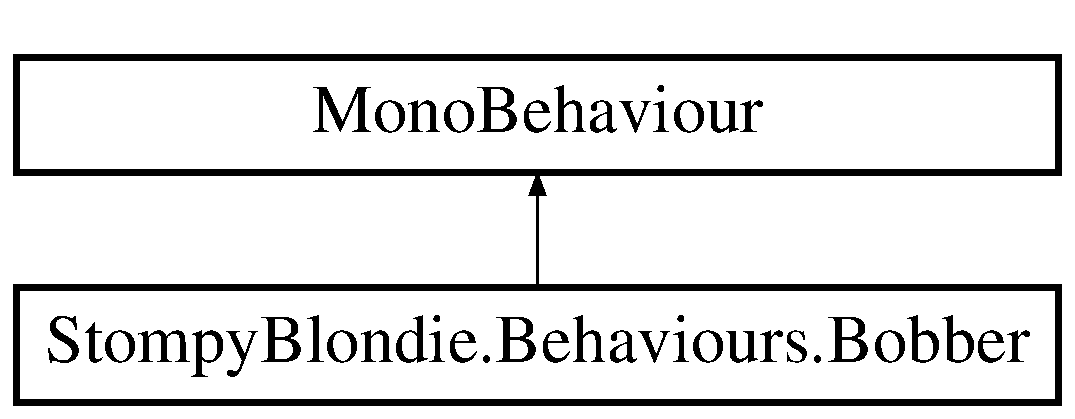
\includegraphics[height=2.000000cm]{class_stompy_blondie_1_1_behaviours_1_1_bobber}
\end{center}
\end{figure}
\subsection*{Public Types}
\begin{DoxyCompactItemize}
\item 
enum \mbox{\hyperlink{class_stompy_blondie_1_1_behaviours_1_1_bobber_aa5824e905d1992e924d9755659a7717e}{Dimension}} \{ \mbox{\hyperlink{class_stompy_blondie_1_1_behaviours_1_1_bobber_aa5824e905d1992e924d9755659a7717ea02129bb861061d1a052c592e2dc6b383}{Dimension.\+X}}, 
\mbox{\hyperlink{class_stompy_blondie_1_1_behaviours_1_1_bobber_aa5824e905d1992e924d9755659a7717ea57cec4137b614c87cb4e24a3d003a3e0}{Dimension.\+Y}}, 
\mbox{\hyperlink{class_stompy_blondie_1_1_behaviours_1_1_bobber_aa5824e905d1992e924d9755659a7717ea21c2e59531c8710156d34a3c30ac81d5}{Dimension.\+Z}}
 \}
\end{DoxyCompactItemize}
\subsection*{Public Member Functions}
\begin{DoxyCompactItemize}
\item 
void \mbox{\hyperlink{class_stompy_blondie_1_1_behaviours_1_1_bobber_aaa2f97e7e7532fc665a6284dd275ba71}{Start}} ()
\item 
void \mbox{\hyperlink{class_stompy_blondie_1_1_behaviours_1_1_bobber_a561d9d22d20aaa4091ed153b866d029c}{Update}} ()
\end{DoxyCompactItemize}
\subsection*{Public Attributes}
\begin{DoxyCompactItemize}
\item 
float \mbox{\hyperlink{class_stompy_blondie_1_1_behaviours_1_1_bobber_af19a43e9b4c27a9f051cb9a2752170b4}{bob\+Distance}}
\item 
\mbox{\hyperlink{class_stompy_blondie_1_1_behaviours_1_1_bobber_aa5824e905d1992e924d9755659a7717e}{Dimension}} \mbox{\hyperlink{class_stompy_blondie_1_1_behaviours_1_1_bobber_a09bd3f72a7af5f83f2c6f6cdd35aeefa}{bob\+Direction}}
\item 
float \mbox{\hyperlink{class_stompy_blondie_1_1_behaviours_1_1_bobber_a70dd7d7f45370459a859ee2c86d5cf9f}{bob\+Speed}} = 1f
\end{DoxyCompactItemize}


\subsection{Member Enumeration Documentation}
\mbox{\Hypertarget{class_stompy_blondie_1_1_behaviours_1_1_bobber_aa5824e905d1992e924d9755659a7717e}\label{class_stompy_blondie_1_1_behaviours_1_1_bobber_aa5824e905d1992e924d9755659a7717e}} 
\index{Stompy\+Blondie\+::\+Behaviours\+::\+Bobber@{Stompy\+Blondie\+::\+Behaviours\+::\+Bobber}!Dimension@{Dimension}}
\index{Dimension@{Dimension}!Stompy\+Blondie\+::\+Behaviours\+::\+Bobber@{Stompy\+Blondie\+::\+Behaviours\+::\+Bobber}}
\subsubsection{\texorpdfstring{Dimension}{Dimension}}
{\footnotesize\ttfamily enum \mbox{\hyperlink{class_stompy_blondie_1_1_behaviours_1_1_bobber_aa5824e905d1992e924d9755659a7717e}{Stompy\+Blondie.\+Behaviours.\+Bobber.\+Dimension}}\hspace{0.3cm}{\ttfamily [strong]}}

\begin{DoxyEnumFields}{Enumerator}
\raisebox{\heightof{T}}[0pt][0pt]{\index{X@{X}!Stompy\+Blondie\+::\+Behaviours\+::\+Bobber@{Stompy\+Blondie\+::\+Behaviours\+::\+Bobber}}\index{Stompy\+Blondie\+::\+Behaviours\+::\+Bobber@{Stompy\+Blondie\+::\+Behaviours\+::\+Bobber}!X@{X}}}\mbox{\Hypertarget{class_stompy_blondie_1_1_behaviours_1_1_bobber_aa5824e905d1992e924d9755659a7717ea02129bb861061d1a052c592e2dc6b383}\label{class_stompy_blondie_1_1_behaviours_1_1_bobber_aa5824e905d1992e924d9755659a7717ea02129bb861061d1a052c592e2dc6b383}} 
X&\\
\hline

\raisebox{\heightof{T}}[0pt][0pt]{\index{Y@{Y}!Stompy\+Blondie\+::\+Behaviours\+::\+Bobber@{Stompy\+Blondie\+::\+Behaviours\+::\+Bobber}}\index{Stompy\+Blondie\+::\+Behaviours\+::\+Bobber@{Stompy\+Blondie\+::\+Behaviours\+::\+Bobber}!Y@{Y}}}\mbox{\Hypertarget{class_stompy_blondie_1_1_behaviours_1_1_bobber_aa5824e905d1992e924d9755659a7717ea57cec4137b614c87cb4e24a3d003a3e0}\label{class_stompy_blondie_1_1_behaviours_1_1_bobber_aa5824e905d1992e924d9755659a7717ea57cec4137b614c87cb4e24a3d003a3e0}} 
Y&\\
\hline

\raisebox{\heightof{T}}[0pt][0pt]{\index{Z@{Z}!Stompy\+Blondie\+::\+Behaviours\+::\+Bobber@{Stompy\+Blondie\+::\+Behaviours\+::\+Bobber}}\index{Stompy\+Blondie\+::\+Behaviours\+::\+Bobber@{Stompy\+Blondie\+::\+Behaviours\+::\+Bobber}!Z@{Z}}}\mbox{\Hypertarget{class_stompy_blondie_1_1_behaviours_1_1_bobber_aa5824e905d1992e924d9755659a7717ea21c2e59531c8710156d34a3c30ac81d5}\label{class_stompy_blondie_1_1_behaviours_1_1_bobber_aa5824e905d1992e924d9755659a7717ea21c2e59531c8710156d34a3c30ac81d5}} 
Z&\\
\hline

\end{DoxyEnumFields}


\subsection{Member Function Documentation}
\mbox{\Hypertarget{class_stompy_blondie_1_1_behaviours_1_1_bobber_aaa2f97e7e7532fc665a6284dd275ba71}\label{class_stompy_blondie_1_1_behaviours_1_1_bobber_aaa2f97e7e7532fc665a6284dd275ba71}} 
\index{Stompy\+Blondie\+::\+Behaviours\+::\+Bobber@{Stompy\+Blondie\+::\+Behaviours\+::\+Bobber}!Start@{Start}}
\index{Start@{Start}!Stompy\+Blondie\+::\+Behaviours\+::\+Bobber@{Stompy\+Blondie\+::\+Behaviours\+::\+Bobber}}
\subsubsection{\texorpdfstring{Start()}{Start()}}
{\footnotesize\ttfamily void Stompy\+Blondie.\+Behaviours.\+Bobber.\+Start (\begin{DoxyParamCaption}{ }\end{DoxyParamCaption})\hspace{0.3cm}{\ttfamily [inline]}}

\mbox{\Hypertarget{class_stompy_blondie_1_1_behaviours_1_1_bobber_a561d9d22d20aaa4091ed153b866d029c}\label{class_stompy_blondie_1_1_behaviours_1_1_bobber_a561d9d22d20aaa4091ed153b866d029c}} 
\index{Stompy\+Blondie\+::\+Behaviours\+::\+Bobber@{Stompy\+Blondie\+::\+Behaviours\+::\+Bobber}!Update@{Update}}
\index{Update@{Update}!Stompy\+Blondie\+::\+Behaviours\+::\+Bobber@{Stompy\+Blondie\+::\+Behaviours\+::\+Bobber}}
\subsubsection{\texorpdfstring{Update()}{Update()}}
{\footnotesize\ttfamily void Stompy\+Blondie.\+Behaviours.\+Bobber.\+Update (\begin{DoxyParamCaption}{ }\end{DoxyParamCaption})\hspace{0.3cm}{\ttfamily [inline]}}



\subsection{Member Data Documentation}
\mbox{\Hypertarget{class_stompy_blondie_1_1_behaviours_1_1_bobber_a09bd3f72a7af5f83f2c6f6cdd35aeefa}\label{class_stompy_blondie_1_1_behaviours_1_1_bobber_a09bd3f72a7af5f83f2c6f6cdd35aeefa}} 
\index{Stompy\+Blondie\+::\+Behaviours\+::\+Bobber@{Stompy\+Blondie\+::\+Behaviours\+::\+Bobber}!bob\+Direction@{bob\+Direction}}
\index{bob\+Direction@{bob\+Direction}!Stompy\+Blondie\+::\+Behaviours\+::\+Bobber@{Stompy\+Blondie\+::\+Behaviours\+::\+Bobber}}
\subsubsection{\texorpdfstring{bob\+Direction}{bobDirection}}
{\footnotesize\ttfamily \mbox{\hyperlink{class_stompy_blondie_1_1_behaviours_1_1_bobber_aa5824e905d1992e924d9755659a7717e}{Dimension}} Stompy\+Blondie.\+Behaviours.\+Bobber.\+bob\+Direction}

\mbox{\Hypertarget{class_stompy_blondie_1_1_behaviours_1_1_bobber_af19a43e9b4c27a9f051cb9a2752170b4}\label{class_stompy_blondie_1_1_behaviours_1_1_bobber_af19a43e9b4c27a9f051cb9a2752170b4}} 
\index{Stompy\+Blondie\+::\+Behaviours\+::\+Bobber@{Stompy\+Blondie\+::\+Behaviours\+::\+Bobber}!bob\+Distance@{bob\+Distance}}
\index{bob\+Distance@{bob\+Distance}!Stompy\+Blondie\+::\+Behaviours\+::\+Bobber@{Stompy\+Blondie\+::\+Behaviours\+::\+Bobber}}
\subsubsection{\texorpdfstring{bob\+Distance}{bobDistance}}
{\footnotesize\ttfamily float Stompy\+Blondie.\+Behaviours.\+Bobber.\+bob\+Distance}

\mbox{\Hypertarget{class_stompy_blondie_1_1_behaviours_1_1_bobber_a70dd7d7f45370459a859ee2c86d5cf9f}\label{class_stompy_blondie_1_1_behaviours_1_1_bobber_a70dd7d7f45370459a859ee2c86d5cf9f}} 
\index{Stompy\+Blondie\+::\+Behaviours\+::\+Bobber@{Stompy\+Blondie\+::\+Behaviours\+::\+Bobber}!bob\+Speed@{bob\+Speed}}
\index{bob\+Speed@{bob\+Speed}!Stompy\+Blondie\+::\+Behaviours\+::\+Bobber@{Stompy\+Blondie\+::\+Behaviours\+::\+Bobber}}
\subsubsection{\texorpdfstring{bob\+Speed}{bobSpeed}}
{\footnotesize\ttfamily float Stompy\+Blondie.\+Behaviours.\+Bobber.\+bob\+Speed = 1f}



The documentation for this class was generated from the following file\+:\begin{DoxyCompactItemize}
\item 
Behaviours/\mbox{\hyperlink{_bobber_8cs}{Bobber.\+cs}}\end{DoxyCompactItemize}

\hypertarget{class_stompy_blondie_1_1_utils_1_1_bone_clone}{}\section{Stompy\+Blondie.\+Utils.\+Bone\+Clone Class Reference}
\label{class_stompy_blondie_1_1_utils_1_1_bone_clone}\index{Stompy\+Blondie.\+Utils.\+Bone\+Clone@{Stompy\+Blondie.\+Utils.\+Bone\+Clone}}
Inheritance diagram for Stompy\+Blondie.\+Utils.\+Bone\+Clone\+:\begin{figure}[H]
\begin{center}
\leavevmode
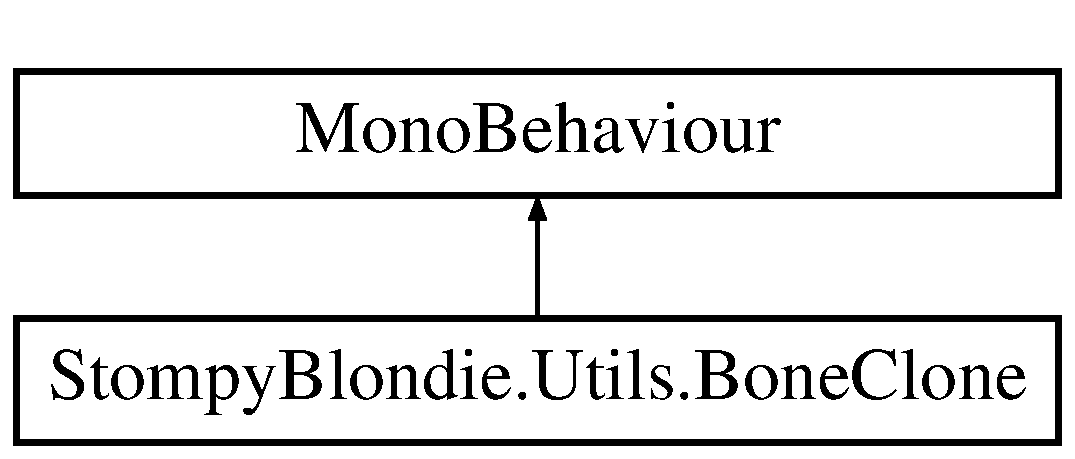
\includegraphics[height=2.000000cm]{class_stompy_blondie_1_1_utils_1_1_bone_clone}
\end{center}
\end{figure}
\subsection*{Public Attributes}
\begin{DoxyCompactItemize}
\item 
Skinned\+Mesh\+Renderer \mbox{\hyperlink{class_stompy_blondie_1_1_utils_1_1_bone_clone_a2003810e13282194ef8aae44d587a9ab}{renderer\+To\+Clone}}
\end{DoxyCompactItemize}


\subsection{Member Data Documentation}
\mbox{\Hypertarget{class_stompy_blondie_1_1_utils_1_1_bone_clone_a2003810e13282194ef8aae44d587a9ab}\label{class_stompy_blondie_1_1_utils_1_1_bone_clone_a2003810e13282194ef8aae44d587a9ab}} 
\index{Stompy\+Blondie\+::\+Utils\+::\+Bone\+Clone@{Stompy\+Blondie\+::\+Utils\+::\+Bone\+Clone}!renderer\+To\+Clone@{renderer\+To\+Clone}}
\index{renderer\+To\+Clone@{renderer\+To\+Clone}!Stompy\+Blondie\+::\+Utils\+::\+Bone\+Clone@{Stompy\+Blondie\+::\+Utils\+::\+Bone\+Clone}}
\subsubsection{\texorpdfstring{renderer\+To\+Clone}{rendererToClone}}
{\footnotesize\ttfamily Skinned\+Mesh\+Renderer Stompy\+Blondie.\+Utils.\+Bone\+Clone.\+renderer\+To\+Clone}



The documentation for this class was generated from the following file\+:\begin{DoxyCompactItemize}
\item 
Utils/\mbox{\hyperlink{_bone_clone_8cs}{Bone\+Clone.\+cs}}\end{DoxyCompactItemize}

\hypertarget{class_stompy_blondie_1_1_systems_1_1_effect}{}\section{Stompy\+Blondie.\+Systems.\+Effect Class Reference}
\label{class_stompy_blondie_1_1_systems_1_1_effect}\index{Stompy\+Blondie.\+Systems.\+Effect@{Stompy\+Blondie.\+Systems.\+Effect}}
\subsection*{Public Member Functions}
\begin{DoxyCompactItemize}
\item 
\mbox{\Hypertarget{class_stompy_blondie_1_1_systems_1_1_effect_af69895e2de62f92bd139e41305ee99a8}\label{class_stompy_blondie_1_1_systems_1_1_effect_af69895e2de62f92bd139e41305ee99a8}} 
{\bfseries Effect} (Game\+Object effect, \mbox{\hyperlink{class_stompy_blondie_1_1_systems_1_1_effects_manager}{Effects\+Manager}} manager)
\item 
\mbox{\Hypertarget{class_stompy_blondie_1_1_systems_1_1_effect_adb4d706c6819eaae1ef1459e60032ff4}\label{class_stompy_blondie_1_1_systems_1_1_effect_adb4d706c6819eaae1ef1459e60032ff4}} 
void {\bfseries Multiply\+Speed} (float factor)
\item 
\mbox{\Hypertarget{class_stompy_blondie_1_1_systems_1_1_effect_a38e13bfc780bf28b651e22f5a2621031}\label{class_stompy_blondie_1_1_systems_1_1_effect_a38e13bfc780bf28b651e22f5a2621031}} 
void {\bfseries Update} ()
\item 
\mbox{\Hypertarget{class_stompy_blondie_1_1_systems_1_1_effect_a23499c024421bfeeb3996d2efd026641}\label{class_stompy_blondie_1_1_systems_1_1_effect_a23499c024421bfeeb3996d2efd026641}} 
void {\bfseries Kill} ()
\end{DoxyCompactItemize}
\subsection*{Public Attributes}
\begin{DoxyCompactItemize}
\item 
\mbox{\Hypertarget{class_stompy_blondie_1_1_systems_1_1_effect_ab5c9c40c7a8df170f1ac8a631dde8e76}\label{class_stompy_blondie_1_1_systems_1_1_effect_ab5c9c40c7a8df170f1ac8a631dde8e76}} 
Game\+Object {\bfseries effect}
\item 
\mbox{\Hypertarget{class_stompy_blondie_1_1_systems_1_1_effect_ad3eb7a90a28a4fbe361214890cdb06b4}\label{class_stompy_blondie_1_1_systems_1_1_effect_ad3eb7a90a28a4fbe361214890cdb06b4}} 
Transform {\bfseries follow\+Transform}
\item 
\mbox{\Hypertarget{class_stompy_blondie_1_1_systems_1_1_effect_a06ce39c8c8192912d9e94a3d337afd4e}\label{class_stompy_blondie_1_1_systems_1_1_effect_a06ce39c8c8192912d9e94a3d337afd4e}} 
\mbox{\hyperlink{class_stompy_blondie_1_1_systems_1_1_effects_manager}{Effects\+Manager}} {\bfseries manager}
\end{DoxyCompactItemize}


The documentation for this class was generated from the following file\+:\begin{DoxyCompactItemize}
\item 
Systems/Effects\+Manager.\+cs\end{DoxyCompactItemize}

\hypertarget{class_stompy_blondie_1_1_systems_1_1_effects_manager}{}\section{Stompy\+Blondie.\+Systems.\+Effects\+Manager Class Reference}
\label{class_stompy_blondie_1_1_systems_1_1_effects_manager}\index{Stompy\+Blondie.\+Systems.\+Effects\+Manager@{Stompy\+Blondie.\+Systems.\+Effects\+Manager}}
Inheritance diagram for Stompy\+Blondie.\+Systems.\+Effects\+Manager\+:\begin{figure}[H]
\begin{center}
\leavevmode
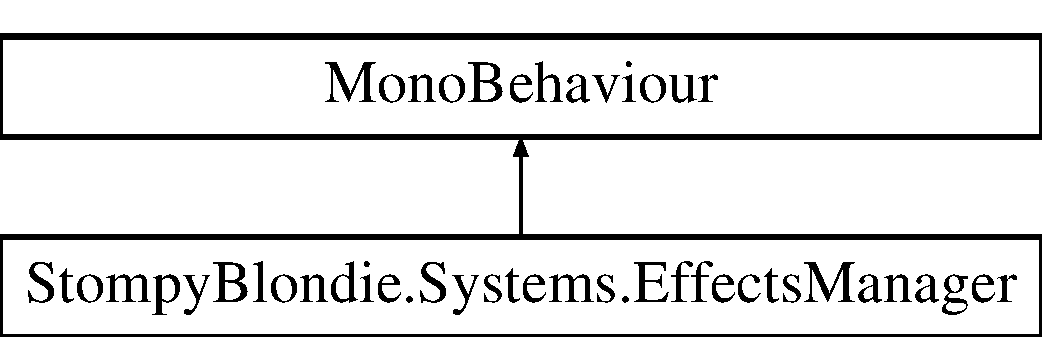
\includegraphics[height=2.000000cm]{class_stompy_blondie_1_1_systems_1_1_effects_manager}
\end{center}
\end{figure}
\subsection*{Public Member Functions}
\begin{DoxyCompactItemize}
\item 
\mbox{\Hypertarget{class_stompy_blondie_1_1_systems_1_1_effects_manager_a168066de1a7b2fb68fe1e8aad700e095}\label{class_stompy_blondie_1_1_systems_1_1_effects_manager_a168066de1a7b2fb68fe1e8aad700e095}} 
void {\bfseries Initialise} (Field\+Info\mbox{[}$\,$\mbox{]} effect\+Types, string effect\+Resources\+Path=\char`\"{}effects/\char`\"{})
\item 
\mbox{\Hypertarget{class_stompy_blondie_1_1_systems_1_1_effects_manager_ac8421abe668767bdca76cfdcc61fc398}\label{class_stompy_blondie_1_1_systems_1_1_effects_manager_ac8421abe668767bdca76cfdcc61fc398}} 
\mbox{\hyperlink{class_stompy_blondie_1_1_systems_1_1_effect}{Effect}} {\bfseries Create\+Effect} (string type, Vector3 location)
\item 
\mbox{\Hypertarget{class_stompy_blondie_1_1_systems_1_1_effects_manager_ab75dc8e99a16fa5950b1e7e95d41f810}\label{class_stompy_blondie_1_1_systems_1_1_effects_manager_ab75dc8e99a16fa5950b1e7e95d41f810}} 
\mbox{\hyperlink{class_stompy_blondie_1_1_systems_1_1_effect}{Effect}} {\bfseries Create\+Effect} (string type, Transform follow)
\item 
\mbox{\Hypertarget{class_stompy_blondie_1_1_systems_1_1_effects_manager_a904acd1941627e0cb611586d220179a9}\label{class_stompy_blondie_1_1_systems_1_1_effects_manager_a904acd1941627e0cb611586d220179a9}} 
void {\bfseries Remove\+Effect} (\mbox{\hyperlink{class_stompy_blondie_1_1_systems_1_1_effect}{Effect}} effect, bool immediate=false)
\end{DoxyCompactItemize}
\subsection*{Static Public Member Functions}
\begin{DoxyCompactItemize}
\item 
\mbox{\Hypertarget{class_stompy_blondie_1_1_systems_1_1_effects_manager_a9c38a685a51d9dafe2b0734a457d6801}\label{class_stompy_blondie_1_1_systems_1_1_effects_manager_a9c38a685a51d9dafe2b0734a457d6801}} 
static \mbox{\hyperlink{class_stompy_blondie_1_1_systems_1_1_effects_manager}{Effects\+Manager}} {\bfseries Create\+Effects\+Manager} (Field\+Info\mbox{[}$\,$\mbox{]} effect\+Types, string effect\+Resources\+Path=\char`\"{}effects/\char`\"{})
\end{DoxyCompactItemize}
\subsection*{Public Attributes}
\begin{DoxyCompactItemize}
\item 
\mbox{\Hypertarget{class_stompy_blondie_1_1_systems_1_1_effects_manager_a9e917930d6e328a83cb87639ac1b3599}\label{class_stompy_blondie_1_1_systems_1_1_effects_manager_a9e917930d6e328a83cb87639ac1b3599}} 
string {\bfseries effect\+Resources\+Path} = \char`\"{}\char`\"{}
\item 
\mbox{\Hypertarget{class_stompy_blondie_1_1_systems_1_1_effects_manager_abde357ddd92a368b4eebc347b5bc3c66}\label{class_stompy_blondie_1_1_systems_1_1_effects_manager_abde357ddd92a368b4eebc347b5bc3c66}} 
Dictionary$<$ string, Game\+Object $>$ {\bfseries preloaded\+Effects}
\item 
\mbox{\Hypertarget{class_stompy_blondie_1_1_systems_1_1_effects_manager_ae66380ec6b74d10b8e3cb2ee8e5fca1e}\label{class_stompy_blondie_1_1_systems_1_1_effects_manager_ae66380ec6b74d10b8e3cb2ee8e5fca1e}} 
List$<$ \mbox{\hyperlink{class_stompy_blondie_1_1_systems_1_1_effect}{Effect}} $>$ {\bfseries active\+Effects}
\item 
\mbox{\Hypertarget{class_stompy_blondie_1_1_systems_1_1_effects_manager_a185cf6e4134d962c94b3ea7e39355339}\label{class_stompy_blondie_1_1_systems_1_1_effects_manager_a185cf6e4134d962c94b3ea7e39355339}} 
Field\+Info \mbox{[}$\,$\mbox{]} {\bfseries effect\+Types}
\end{DoxyCompactItemize}


The documentation for this class was generated from the following file\+:\begin{DoxyCompactItemize}
\item 
Systems/Effects\+Manager.\+cs\end{DoxyCompactItemize}

\hypertarget{class_stompy_blondie_1_1_extensions_1_1_extension_mono_behaviour}{}\section{Stompy\+Blondie.\+Extensions.\+Extension\+Mono\+Behaviour Class Reference}
\label{class_stompy_blondie_1_1_extensions_1_1_extension_mono_behaviour}\index{Stompy\+Blondie.\+Extensions.\+Extension\+Mono\+Behaviour@{Stompy\+Blondie.\+Extensions.\+Extension\+Mono\+Behaviour}}
Inheritance diagram for Stompy\+Blondie.\+Extensions.\+Extension\+Mono\+Behaviour\+:\begin{figure}[H]
\begin{center}
\leavevmode
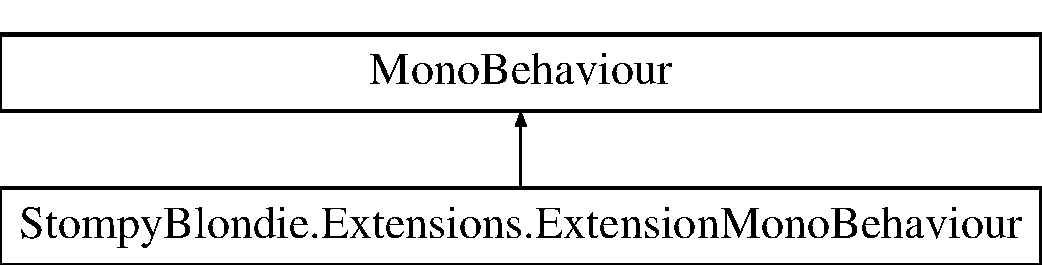
\includegraphics[height=2.000000cm]{class_stompy_blondie_1_1_extensions_1_1_extension_mono_behaviour}
\end{center}
\end{figure}
\subsection*{Static Public Member Functions}
\begin{DoxyCompactItemize}
\item 
\mbox{\Hypertarget{class_stompy_blondie_1_1_extensions_1_1_extension_mono_behaviour_a472cd1f5e863bf9d36b7a455167f2b97}\label{class_stompy_blondie_1_1_extensions_1_1_extension_mono_behaviour_a472cd1f5e863bf9d36b7a455167f2b97}} 
static \mbox{\hyperlink{class_stompy_blondie_1_1_extensions_1_1_extension_mono_behaviour}{Extension\+Mono\+Behaviour}} {\bfseries Get\+Instance} ()
\end{DoxyCompactItemize}


The documentation for this class was generated from the following file\+:\begin{DoxyCompactItemize}
\item 
Extensions/Extension\+Mono\+Behaviour.\+cs\end{DoxyCompactItemize}

\hypertarget{class_stompy_blondie_1_1_behaviours_1_1_face_camera}{}\section{Stompy\+Blondie.\+Behaviours.\+Face\+Camera Class Reference}
\label{class_stompy_blondie_1_1_behaviours_1_1_face_camera}\index{Stompy\+Blondie.\+Behaviours.\+Face\+Camera@{Stompy\+Blondie.\+Behaviours.\+Face\+Camera}}
Inheritance diagram for Stompy\+Blondie.\+Behaviours.\+Face\+Camera\+:\begin{figure}[H]
\begin{center}
\leavevmode
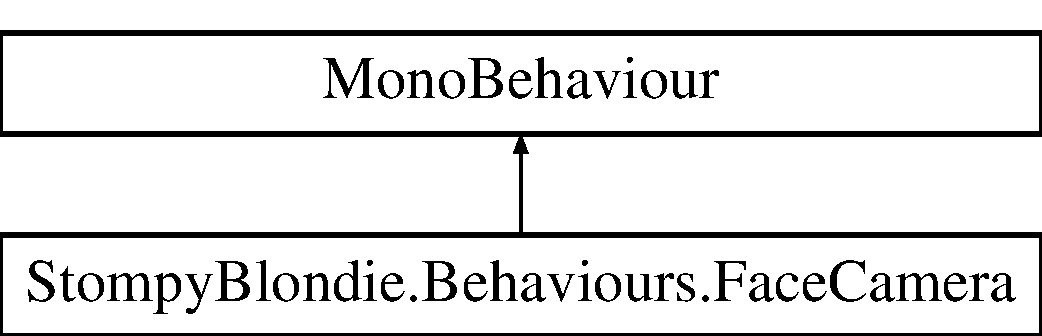
\includegraphics[height=2.000000cm]{class_stompy_blondie_1_1_behaviours_1_1_face_camera}
\end{center}
\end{figure}


The documentation for this class was generated from the following file\+:\begin{DoxyCompactItemize}
\item 
Behaviours/Face\+Camera.\+cs\end{DoxyCompactItemize}

\hypertarget{class_stompy_blondie_1_1_behaviours_1_1_is_mouse_over}{}\section{Stompy\+Blondie.\+Behaviours.\+Is\+Mouse\+Over Class Reference}
\label{class_stompy_blondie_1_1_behaviours_1_1_is_mouse_over}\index{Stompy\+Blondie.\+Behaviours.\+Is\+Mouse\+Over@{Stompy\+Blondie.\+Behaviours.\+Is\+Mouse\+Over}}
Inheritance diagram for Stompy\+Blondie.\+Behaviours.\+Is\+Mouse\+Over\+:\begin{figure}[H]
\begin{center}
\leavevmode
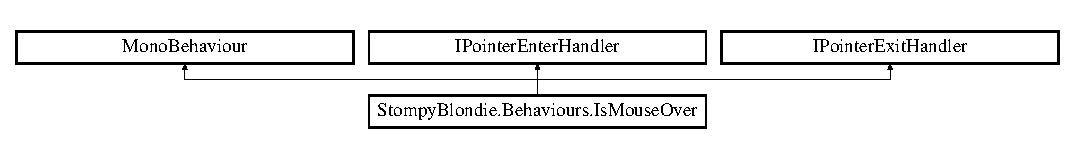
\includegraphics[height=1.487384cm]{class_stompy_blondie_1_1_behaviours_1_1_is_mouse_over}
\end{center}
\end{figure}
\subsection*{Public Member Functions}
\begin{DoxyCompactItemize}
\item 
void \mbox{\hyperlink{class_stompy_blondie_1_1_behaviours_1_1_is_mouse_over_ad8eda7c464bd30cf1104447052e04e32}{On\+Pointer\+Enter}} (Pointer\+Event\+Data event\+Data)
\item 
void \mbox{\hyperlink{class_stompy_blondie_1_1_behaviours_1_1_is_mouse_over_ad624ad1de28269173b245a8456d34ef8}{On\+Pointer\+Exit}} (Pointer\+Event\+Data event\+Data)
\end{DoxyCompactItemize}
\subsection*{Public Attributes}
\begin{DoxyCompactItemize}
\item 
bool \mbox{\hyperlink{class_stompy_blondie_1_1_behaviours_1_1_is_mouse_over_a4b31cf2a692c0cdf41c04d399a70c332}{is\+Over}} = false
\end{DoxyCompactItemize}


\subsection{Member Function Documentation}
\mbox{\Hypertarget{class_stompy_blondie_1_1_behaviours_1_1_is_mouse_over_ad8eda7c464bd30cf1104447052e04e32}\label{class_stompy_blondie_1_1_behaviours_1_1_is_mouse_over_ad8eda7c464bd30cf1104447052e04e32}} 
\index{Stompy\+Blondie\+::\+Behaviours\+::\+Is\+Mouse\+Over@{Stompy\+Blondie\+::\+Behaviours\+::\+Is\+Mouse\+Over}!On\+Pointer\+Enter@{On\+Pointer\+Enter}}
\index{On\+Pointer\+Enter@{On\+Pointer\+Enter}!Stompy\+Blondie\+::\+Behaviours\+::\+Is\+Mouse\+Over@{Stompy\+Blondie\+::\+Behaviours\+::\+Is\+Mouse\+Over}}
\subsubsection{\texorpdfstring{On\+Pointer\+Enter()}{OnPointerEnter()}}
{\footnotesize\ttfamily void Stompy\+Blondie.\+Behaviours.\+Is\+Mouse\+Over.\+On\+Pointer\+Enter (\begin{DoxyParamCaption}\item[{Pointer\+Event\+Data}]{event\+Data }\end{DoxyParamCaption})\hspace{0.3cm}{\ttfamily [inline]}}

\mbox{\Hypertarget{class_stompy_blondie_1_1_behaviours_1_1_is_mouse_over_ad624ad1de28269173b245a8456d34ef8}\label{class_stompy_blondie_1_1_behaviours_1_1_is_mouse_over_ad624ad1de28269173b245a8456d34ef8}} 
\index{Stompy\+Blondie\+::\+Behaviours\+::\+Is\+Mouse\+Over@{Stompy\+Blondie\+::\+Behaviours\+::\+Is\+Mouse\+Over}!On\+Pointer\+Exit@{On\+Pointer\+Exit}}
\index{On\+Pointer\+Exit@{On\+Pointer\+Exit}!Stompy\+Blondie\+::\+Behaviours\+::\+Is\+Mouse\+Over@{Stompy\+Blondie\+::\+Behaviours\+::\+Is\+Mouse\+Over}}
\subsubsection{\texorpdfstring{On\+Pointer\+Exit()}{OnPointerExit()}}
{\footnotesize\ttfamily void Stompy\+Blondie.\+Behaviours.\+Is\+Mouse\+Over.\+On\+Pointer\+Exit (\begin{DoxyParamCaption}\item[{Pointer\+Event\+Data}]{event\+Data }\end{DoxyParamCaption})\hspace{0.3cm}{\ttfamily [inline]}}



\subsection{Member Data Documentation}
\mbox{\Hypertarget{class_stompy_blondie_1_1_behaviours_1_1_is_mouse_over_a4b31cf2a692c0cdf41c04d399a70c332}\label{class_stompy_blondie_1_1_behaviours_1_1_is_mouse_over_a4b31cf2a692c0cdf41c04d399a70c332}} 
\index{Stompy\+Blondie\+::\+Behaviours\+::\+Is\+Mouse\+Over@{Stompy\+Blondie\+::\+Behaviours\+::\+Is\+Mouse\+Over}!is\+Over@{is\+Over}}
\index{is\+Over@{is\+Over}!Stompy\+Blondie\+::\+Behaviours\+::\+Is\+Mouse\+Over@{Stompy\+Blondie\+::\+Behaviours\+::\+Is\+Mouse\+Over}}
\subsubsection{\texorpdfstring{is\+Over}{isOver}}
{\footnotesize\ttfamily bool Stompy\+Blondie.\+Behaviours.\+Is\+Mouse\+Over.\+is\+Over = false}



The documentation for this class was generated from the following file\+:\begin{DoxyCompactItemize}
\item 
Behaviours/\mbox{\hyperlink{_is_mouse_over_8cs}{Is\+Mouse\+Over.\+cs}}\end{DoxyCompactItemize}

\hypertarget{class_stompy_blondie_1_1_a_i_1_1_navigation_map}{}\section{Stompy\+Blondie.\+A\+I.\+Navigation\+Map Class Reference}
\label{class_stompy_blondie_1_1_a_i_1_1_navigation_map}\index{Stompy\+Blondie.\+A\+I.\+Navigation\+Map@{Stompy\+Blondie.\+A\+I.\+Navigation\+Map}}
\subsection*{Public Member Functions}
\begin{DoxyCompactItemize}
\item 
\mbox{\hyperlink{class_stompy_blondie_1_1_a_i_1_1_navigation_map_a0e5a432873f28ea782cb925c36610815}{Navigation\+Map}} ()
\item 
\mbox{\hyperlink{class_stompy_blondie_1_1_a_i_1_1_navigation_map_a62f3061cd8d46288f7fee1e6c80a1b9b}{Navigation\+Map}} (\mbox{\hyperlink{class_stompy_blondie_1_1_a_i_1_1_navigation_map}{Navigation\+Map}} clone\+From)
\item 
void \mbox{\hyperlink{class_stompy_blondie_1_1_a_i_1_1_navigation_map_a5922bcfcb17953ec21c868b260b41953}{Reset}} ()
\item 
bool \mbox{\hyperlink{class_stompy_blondie_1_1_a_i_1_1_navigation_map_a10c2593b8a9fbaf0ac01095f40c12dc8}{Has\+Point}} (\mbox{\hyperlink{struct_stompy_blondie_1_1_common_1_1_types_1_1_pos}{Pos}} position)
\item 
bool \mbox{\hyperlink{class_stompy_blondie_1_1_a_i_1_1_navigation_map_af6d4dcdcca40f142146538ed2fe7c21f}{Add\+Point}} (\mbox{\hyperlink{struct_stompy_blondie_1_1_common_1_1_types_1_1_pos}{Pos}} position)
\item 
bool \mbox{\hyperlink{class_stompy_blondie_1_1_a_i_1_1_navigation_map_a2658ca4206a19449243d4a16393ebb85}{Add\+Point\+Link}} (\mbox{\hyperlink{struct_stompy_blondie_1_1_common_1_1_types_1_1_pos}{Pos}} pointA, \mbox{\hyperlink{struct_stompy_blondie_1_1_common_1_1_types_1_1_pos}{Pos}} pointB, float cost\+Multiplier=1f)
\item 
void \mbox{\hyperlink{class_stompy_blondie_1_1_a_i_1_1_navigation_map_ae13b0ae98c3b2309b0349439bf58ed13}{Remove\+Point}} (\mbox{\hyperlink{struct_stompy_blondie_1_1_common_1_1_types_1_1_pos}{Pos}} position)
\item 
void \mbox{\hyperlink{class_stompy_blondie_1_1_a_i_1_1_navigation_map_aa49f9eb7f626fad4bbbb9ddd411fa41d}{Break\+Point\+Link}} (\mbox{\hyperlink{struct_stompy_blondie_1_1_common_1_1_types_1_1_pos}{Pos}} pointA, \mbox{\hyperlink{struct_stompy_blondie_1_1_common_1_1_types_1_1_pos}{Pos}} pointB)
\item 
float \mbox{\hyperlink{class_stompy_blondie_1_1_a_i_1_1_navigation_map_a0ce1fac02a5a31b904baada6aff83bcd}{Distance\+Between\+Points}} (\mbox{\hyperlink{struct_stompy_blondie_1_1_common_1_1_types_1_1_pos}{Pos}} pointA, \mbox{\hyperlink{struct_stompy_blondie_1_1_common_1_1_types_1_1_pos}{Pos}} pointB)
\item 
bool \mbox{\hyperlink{class_stompy_blondie_1_1_a_i_1_1_navigation_map_a059f94fa6e73419756517f761f2bb3f5}{Superimpose\+Navigation\+Map}} (\mbox{\hyperlink{class_stompy_blondie_1_1_a_i_1_1_navigation_map}{Navigation\+Map}} nav\+Map, \mbox{\hyperlink{struct_stompy_blondie_1_1_common_1_1_types_1_1_pos}{Pos}} position, \mbox{\hyperlink{namespace_stompy_blondie_1_1_common_1_1_types_a67d21ccf6a23cdea91c271cce76f920f}{Eight\+Direction}} direction)
\end{DoxyCompactItemize}
\subsection*{Public Attributes}
\begin{DoxyCompactItemize}
\item 
Dictionary$<$ \mbox{\hyperlink{struct_stompy_blondie_1_1_common_1_1_types_1_1_pos}{Pos}}, \mbox{\hyperlink{struct_stompy_blondie_1_1_a_i_1_1_navigation_point}{Navigation\+Point}} $>$ \mbox{\hyperlink{class_stompy_blondie_1_1_a_i_1_1_navigation_map_af4f71225b8d491f23974e2b4cf2d18e9}{points}} = new Dictionary$<$\mbox{\hyperlink{struct_stompy_blondie_1_1_common_1_1_types_1_1_pos}{Pos}}, \mbox{\hyperlink{struct_stompy_blondie_1_1_a_i_1_1_navigation_point}{Navigation\+Point}}$>$()
\item 
float \mbox{\hyperlink{class_stompy_blondie_1_1_a_i_1_1_navigation_map_a2db7ec95521970ba1e2eafbeaf3418fc}{minX}}
\end{DoxyCompactItemize}


\subsection{Constructor \& Destructor Documentation}
\mbox{\Hypertarget{class_stompy_blondie_1_1_a_i_1_1_navigation_map_a0e5a432873f28ea782cb925c36610815}\label{class_stompy_blondie_1_1_a_i_1_1_navigation_map_a0e5a432873f28ea782cb925c36610815}} 
\index{Stompy\+Blondie\+::\+A\+I\+::\+Navigation\+Map@{Stompy\+Blondie\+::\+A\+I\+::\+Navigation\+Map}!Navigation\+Map@{Navigation\+Map}}
\index{Navigation\+Map@{Navigation\+Map}!Stompy\+Blondie\+::\+A\+I\+::\+Navigation\+Map@{Stompy\+Blondie\+::\+A\+I\+::\+Navigation\+Map}}
\subsubsection{\texorpdfstring{Navigation\+Map()}{NavigationMap()}\hspace{0.1cm}{\footnotesize\ttfamily [1/2]}}
{\footnotesize\ttfamily Stompy\+Blondie.\+A\+I.\+Navigation\+Map.\+Navigation\+Map (\begin{DoxyParamCaption}{ }\end{DoxyParamCaption})\hspace{0.3cm}{\ttfamily [inline]}}

\mbox{\Hypertarget{class_stompy_blondie_1_1_a_i_1_1_navigation_map_a62f3061cd8d46288f7fee1e6c80a1b9b}\label{class_stompy_blondie_1_1_a_i_1_1_navigation_map_a62f3061cd8d46288f7fee1e6c80a1b9b}} 
\index{Stompy\+Blondie\+::\+A\+I\+::\+Navigation\+Map@{Stompy\+Blondie\+::\+A\+I\+::\+Navigation\+Map}!Navigation\+Map@{Navigation\+Map}}
\index{Navigation\+Map@{Navigation\+Map}!Stompy\+Blondie\+::\+A\+I\+::\+Navigation\+Map@{Stompy\+Blondie\+::\+A\+I\+::\+Navigation\+Map}}
\subsubsection{\texorpdfstring{Navigation\+Map()}{NavigationMap()}\hspace{0.1cm}{\footnotesize\ttfamily [2/2]}}
{\footnotesize\ttfamily Stompy\+Blondie.\+A\+I.\+Navigation\+Map.\+Navigation\+Map (\begin{DoxyParamCaption}\item[{\mbox{\hyperlink{class_stompy_blondie_1_1_a_i_1_1_navigation_map}{Navigation\+Map}}}]{clone\+From }\end{DoxyParamCaption})\hspace{0.3cm}{\ttfamily [inline]}}



\subsection{Member Function Documentation}
\mbox{\Hypertarget{class_stompy_blondie_1_1_a_i_1_1_navigation_map_af6d4dcdcca40f142146538ed2fe7c21f}\label{class_stompy_blondie_1_1_a_i_1_1_navigation_map_af6d4dcdcca40f142146538ed2fe7c21f}} 
\index{Stompy\+Blondie\+::\+A\+I\+::\+Navigation\+Map@{Stompy\+Blondie\+::\+A\+I\+::\+Navigation\+Map}!Add\+Point@{Add\+Point}}
\index{Add\+Point@{Add\+Point}!Stompy\+Blondie\+::\+A\+I\+::\+Navigation\+Map@{Stompy\+Blondie\+::\+A\+I\+::\+Navigation\+Map}}
\subsubsection{\texorpdfstring{Add\+Point()}{AddPoint()}}
{\footnotesize\ttfamily bool Stompy\+Blondie.\+A\+I.\+Navigation\+Map.\+Add\+Point (\begin{DoxyParamCaption}\item[{\mbox{\hyperlink{struct_stompy_blondie_1_1_common_1_1_types_1_1_pos}{Pos}}}]{position }\end{DoxyParamCaption})\hspace{0.3cm}{\ttfamily [inline]}}

\mbox{\Hypertarget{class_stompy_blondie_1_1_a_i_1_1_navigation_map_a2658ca4206a19449243d4a16393ebb85}\label{class_stompy_blondie_1_1_a_i_1_1_navigation_map_a2658ca4206a19449243d4a16393ebb85}} 
\index{Stompy\+Blondie\+::\+A\+I\+::\+Navigation\+Map@{Stompy\+Blondie\+::\+A\+I\+::\+Navigation\+Map}!Add\+Point\+Link@{Add\+Point\+Link}}
\index{Add\+Point\+Link@{Add\+Point\+Link}!Stompy\+Blondie\+::\+A\+I\+::\+Navigation\+Map@{Stompy\+Blondie\+::\+A\+I\+::\+Navigation\+Map}}
\subsubsection{\texorpdfstring{Add\+Point\+Link()}{AddPointLink()}}
{\footnotesize\ttfamily bool Stompy\+Blondie.\+A\+I.\+Navigation\+Map.\+Add\+Point\+Link (\begin{DoxyParamCaption}\item[{\mbox{\hyperlink{struct_stompy_blondie_1_1_common_1_1_types_1_1_pos}{Pos}}}]{pointA,  }\item[{\mbox{\hyperlink{struct_stompy_blondie_1_1_common_1_1_types_1_1_pos}{Pos}}}]{pointB,  }\item[{float}]{cost\+Multiplier = {\ttfamily 1f} }\end{DoxyParamCaption})\hspace{0.3cm}{\ttfamily [inline]}}

\mbox{\Hypertarget{class_stompy_blondie_1_1_a_i_1_1_navigation_map_aa49f9eb7f626fad4bbbb9ddd411fa41d}\label{class_stompy_blondie_1_1_a_i_1_1_navigation_map_aa49f9eb7f626fad4bbbb9ddd411fa41d}} 
\index{Stompy\+Blondie\+::\+A\+I\+::\+Navigation\+Map@{Stompy\+Blondie\+::\+A\+I\+::\+Navigation\+Map}!Break\+Point\+Link@{Break\+Point\+Link}}
\index{Break\+Point\+Link@{Break\+Point\+Link}!Stompy\+Blondie\+::\+A\+I\+::\+Navigation\+Map@{Stompy\+Blondie\+::\+A\+I\+::\+Navigation\+Map}}
\subsubsection{\texorpdfstring{Break\+Point\+Link()}{BreakPointLink()}}
{\footnotesize\ttfamily void Stompy\+Blondie.\+A\+I.\+Navigation\+Map.\+Break\+Point\+Link (\begin{DoxyParamCaption}\item[{\mbox{\hyperlink{struct_stompy_blondie_1_1_common_1_1_types_1_1_pos}{Pos}}}]{pointA,  }\item[{\mbox{\hyperlink{struct_stompy_blondie_1_1_common_1_1_types_1_1_pos}{Pos}}}]{pointB }\end{DoxyParamCaption})\hspace{0.3cm}{\ttfamily [inline]}}

\mbox{\Hypertarget{class_stompy_blondie_1_1_a_i_1_1_navigation_map_a0ce1fac02a5a31b904baada6aff83bcd}\label{class_stompy_blondie_1_1_a_i_1_1_navigation_map_a0ce1fac02a5a31b904baada6aff83bcd}} 
\index{Stompy\+Blondie\+::\+A\+I\+::\+Navigation\+Map@{Stompy\+Blondie\+::\+A\+I\+::\+Navigation\+Map}!Distance\+Between\+Points@{Distance\+Between\+Points}}
\index{Distance\+Between\+Points@{Distance\+Between\+Points}!Stompy\+Blondie\+::\+A\+I\+::\+Navigation\+Map@{Stompy\+Blondie\+::\+A\+I\+::\+Navigation\+Map}}
\subsubsection{\texorpdfstring{Distance\+Between\+Points()}{DistanceBetweenPoints()}}
{\footnotesize\ttfamily float Stompy\+Blondie.\+A\+I.\+Navigation\+Map.\+Distance\+Between\+Points (\begin{DoxyParamCaption}\item[{\mbox{\hyperlink{struct_stompy_blondie_1_1_common_1_1_types_1_1_pos}{Pos}}}]{pointA,  }\item[{\mbox{\hyperlink{struct_stompy_blondie_1_1_common_1_1_types_1_1_pos}{Pos}}}]{pointB }\end{DoxyParamCaption})\hspace{0.3cm}{\ttfamily [inline]}}

\mbox{\Hypertarget{class_stompy_blondie_1_1_a_i_1_1_navigation_map_a10c2593b8a9fbaf0ac01095f40c12dc8}\label{class_stompy_blondie_1_1_a_i_1_1_navigation_map_a10c2593b8a9fbaf0ac01095f40c12dc8}} 
\index{Stompy\+Blondie\+::\+A\+I\+::\+Navigation\+Map@{Stompy\+Blondie\+::\+A\+I\+::\+Navigation\+Map}!Has\+Point@{Has\+Point}}
\index{Has\+Point@{Has\+Point}!Stompy\+Blondie\+::\+A\+I\+::\+Navigation\+Map@{Stompy\+Blondie\+::\+A\+I\+::\+Navigation\+Map}}
\subsubsection{\texorpdfstring{Has\+Point()}{HasPoint()}}
{\footnotesize\ttfamily bool Stompy\+Blondie.\+A\+I.\+Navigation\+Map.\+Has\+Point (\begin{DoxyParamCaption}\item[{\mbox{\hyperlink{struct_stompy_blondie_1_1_common_1_1_types_1_1_pos}{Pos}}}]{position }\end{DoxyParamCaption})\hspace{0.3cm}{\ttfamily [inline]}}

\mbox{\Hypertarget{class_stompy_blondie_1_1_a_i_1_1_navigation_map_ae13b0ae98c3b2309b0349439bf58ed13}\label{class_stompy_blondie_1_1_a_i_1_1_navigation_map_ae13b0ae98c3b2309b0349439bf58ed13}} 
\index{Stompy\+Blondie\+::\+A\+I\+::\+Navigation\+Map@{Stompy\+Blondie\+::\+A\+I\+::\+Navigation\+Map}!Remove\+Point@{Remove\+Point}}
\index{Remove\+Point@{Remove\+Point}!Stompy\+Blondie\+::\+A\+I\+::\+Navigation\+Map@{Stompy\+Blondie\+::\+A\+I\+::\+Navigation\+Map}}
\subsubsection{\texorpdfstring{Remove\+Point()}{RemovePoint()}}
{\footnotesize\ttfamily void Stompy\+Blondie.\+A\+I.\+Navigation\+Map.\+Remove\+Point (\begin{DoxyParamCaption}\item[{\mbox{\hyperlink{struct_stompy_blondie_1_1_common_1_1_types_1_1_pos}{Pos}}}]{position }\end{DoxyParamCaption})\hspace{0.3cm}{\ttfamily [inline]}}

\mbox{\Hypertarget{class_stompy_blondie_1_1_a_i_1_1_navigation_map_a5922bcfcb17953ec21c868b260b41953}\label{class_stompy_blondie_1_1_a_i_1_1_navigation_map_a5922bcfcb17953ec21c868b260b41953}} 
\index{Stompy\+Blondie\+::\+A\+I\+::\+Navigation\+Map@{Stompy\+Blondie\+::\+A\+I\+::\+Navigation\+Map}!Reset@{Reset}}
\index{Reset@{Reset}!Stompy\+Blondie\+::\+A\+I\+::\+Navigation\+Map@{Stompy\+Blondie\+::\+A\+I\+::\+Navigation\+Map}}
\subsubsection{\texorpdfstring{Reset()}{Reset()}}
{\footnotesize\ttfamily void Stompy\+Blondie.\+A\+I.\+Navigation\+Map.\+Reset (\begin{DoxyParamCaption}{ }\end{DoxyParamCaption})\hspace{0.3cm}{\ttfamily [inline]}}

\mbox{\Hypertarget{class_stompy_blondie_1_1_a_i_1_1_navigation_map_a059f94fa6e73419756517f761f2bb3f5}\label{class_stompy_blondie_1_1_a_i_1_1_navigation_map_a059f94fa6e73419756517f761f2bb3f5}} 
\index{Stompy\+Blondie\+::\+A\+I\+::\+Navigation\+Map@{Stompy\+Blondie\+::\+A\+I\+::\+Navigation\+Map}!Superimpose\+Navigation\+Map@{Superimpose\+Navigation\+Map}}
\index{Superimpose\+Navigation\+Map@{Superimpose\+Navigation\+Map}!Stompy\+Blondie\+::\+A\+I\+::\+Navigation\+Map@{Stompy\+Blondie\+::\+A\+I\+::\+Navigation\+Map}}
\subsubsection{\texorpdfstring{Superimpose\+Navigation\+Map()}{SuperimposeNavigationMap()}}
{\footnotesize\ttfamily bool Stompy\+Blondie.\+A\+I.\+Navigation\+Map.\+Superimpose\+Navigation\+Map (\begin{DoxyParamCaption}\item[{\mbox{\hyperlink{class_stompy_blondie_1_1_a_i_1_1_navigation_map}{Navigation\+Map}}}]{nav\+Map,  }\item[{\mbox{\hyperlink{struct_stompy_blondie_1_1_common_1_1_types_1_1_pos}{Pos}}}]{position,  }\item[{\mbox{\hyperlink{namespace_stompy_blondie_1_1_common_1_1_types_a67d21ccf6a23cdea91c271cce76f920f}{Eight\+Direction}}}]{direction }\end{DoxyParamCaption})\hspace{0.3cm}{\ttfamily [inline]}}



\subsection{Member Data Documentation}
\mbox{\Hypertarget{class_stompy_blondie_1_1_a_i_1_1_navigation_map_a2db7ec95521970ba1e2eafbeaf3418fc}\label{class_stompy_blondie_1_1_a_i_1_1_navigation_map_a2db7ec95521970ba1e2eafbeaf3418fc}} 
\index{Stompy\+Blondie\+::\+A\+I\+::\+Navigation\+Map@{Stompy\+Blondie\+::\+A\+I\+::\+Navigation\+Map}!minX@{minX}}
\index{minX@{minX}!Stompy\+Blondie\+::\+A\+I\+::\+Navigation\+Map@{Stompy\+Blondie\+::\+A\+I\+::\+Navigation\+Map}}
\subsubsection{\texorpdfstring{minX}{minX}}
{\footnotesize\ttfamily float Stompy\+Blondie.\+A\+I.\+Navigation\+Map.\+minX}

\mbox{\Hypertarget{class_stompy_blondie_1_1_a_i_1_1_navigation_map_af4f71225b8d491f23974e2b4cf2d18e9}\label{class_stompy_blondie_1_1_a_i_1_1_navigation_map_af4f71225b8d491f23974e2b4cf2d18e9}} 
\index{Stompy\+Blondie\+::\+A\+I\+::\+Navigation\+Map@{Stompy\+Blondie\+::\+A\+I\+::\+Navigation\+Map}!points@{points}}
\index{points@{points}!Stompy\+Blondie\+::\+A\+I\+::\+Navigation\+Map@{Stompy\+Blondie\+::\+A\+I\+::\+Navigation\+Map}}
\subsubsection{\texorpdfstring{points}{points}}
{\footnotesize\ttfamily Dictionary$<$\mbox{\hyperlink{struct_stompy_blondie_1_1_common_1_1_types_1_1_pos}{Pos}}, \mbox{\hyperlink{struct_stompy_blondie_1_1_a_i_1_1_navigation_point}{Navigation\+Point}}$>$ Stompy\+Blondie.\+A\+I.\+Navigation\+Map.\+points = new Dictionary$<$\mbox{\hyperlink{struct_stompy_blondie_1_1_common_1_1_types_1_1_pos}{Pos}}, \mbox{\hyperlink{struct_stompy_blondie_1_1_a_i_1_1_navigation_point}{Navigation\+Point}}$>$()}



The documentation for this class was generated from the following file\+:\begin{DoxyCompactItemize}
\item 
A\+I/\mbox{\hyperlink{_tilemap_navigation_8cs}{Tilemap\+Navigation.\+cs}}\end{DoxyCompactItemize}

\hypertarget{class_stompy_blondie_1_1_a_i_1_1_navigation_map_debug_renderer}{}\section{Stompy\+Blondie.\+A\+I.\+Navigation\+Map\+Debug\+Renderer Class Reference}
\label{class_stompy_blondie_1_1_a_i_1_1_navigation_map_debug_renderer}\index{Stompy\+Blondie.\+A\+I.\+Navigation\+Map\+Debug\+Renderer@{Stompy\+Blondie.\+A\+I.\+Navigation\+Map\+Debug\+Renderer}}
Inheritance diagram for Stompy\+Blondie.\+A\+I.\+Navigation\+Map\+Debug\+Renderer\+:\begin{figure}[H]
\begin{center}
\leavevmode
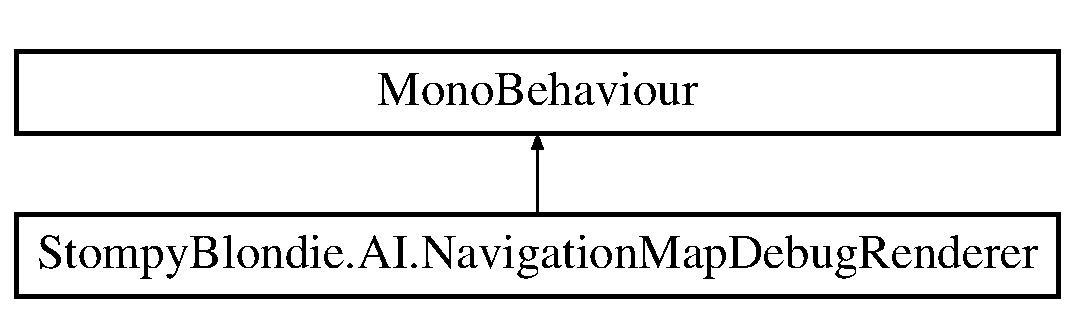
\includegraphics[height=2.000000cm]{class_stompy_blondie_1_1_a_i_1_1_navigation_map_debug_renderer}
\end{center}
\end{figure}
\subsection*{Public Attributes}
\begin{DoxyCompactItemize}
\item 
\mbox{\hyperlink{class_stompy_blondie_1_1_a_i_1_1_navigation_map}{Navigation\+Map}} \mbox{\hyperlink{class_stompy_blondie_1_1_a_i_1_1_navigation_map_debug_renderer_a0a77ce86000ac6b86e4c703876811f16}{navigation\+Map}}
\item 
float \mbox{\hyperlink{class_stompy_blondie_1_1_a_i_1_1_navigation_map_debug_renderer_acd8a0a421c1a96bfb97b60096393f272}{Size\+Of\+Nav\+Points}} = .\+01f
\item 
float \mbox{\hyperlink{class_stompy_blondie_1_1_a_i_1_1_navigation_map_debug_renderer_a7ed34eb6c899be86811aa39b64152242}{scale}} = 1f
\item 
Vector3 \mbox{\hyperlink{class_stompy_blondie_1_1_a_i_1_1_navigation_map_debug_renderer_aaf4d2f24bdea73fbb609397acfacbd92}{offset}}
\end{DoxyCompactItemize}


\subsection{Member Data Documentation}
\mbox{\Hypertarget{class_stompy_blondie_1_1_a_i_1_1_navigation_map_debug_renderer_a0a77ce86000ac6b86e4c703876811f16}\label{class_stompy_blondie_1_1_a_i_1_1_navigation_map_debug_renderer_a0a77ce86000ac6b86e4c703876811f16}} 
\index{Stompy\+Blondie\+::\+A\+I\+::\+Navigation\+Map\+Debug\+Renderer@{Stompy\+Blondie\+::\+A\+I\+::\+Navigation\+Map\+Debug\+Renderer}!navigation\+Map@{navigation\+Map}}
\index{navigation\+Map@{navigation\+Map}!Stompy\+Blondie\+::\+A\+I\+::\+Navigation\+Map\+Debug\+Renderer@{Stompy\+Blondie\+::\+A\+I\+::\+Navigation\+Map\+Debug\+Renderer}}
\subsubsection{\texorpdfstring{navigation\+Map}{navigationMap}}
{\footnotesize\ttfamily \mbox{\hyperlink{class_stompy_blondie_1_1_a_i_1_1_navigation_map}{Navigation\+Map}} Stompy\+Blondie.\+A\+I.\+Navigation\+Map\+Debug\+Renderer.\+navigation\+Map}

\mbox{\Hypertarget{class_stompy_blondie_1_1_a_i_1_1_navigation_map_debug_renderer_aaf4d2f24bdea73fbb609397acfacbd92}\label{class_stompy_blondie_1_1_a_i_1_1_navigation_map_debug_renderer_aaf4d2f24bdea73fbb609397acfacbd92}} 
\index{Stompy\+Blondie\+::\+A\+I\+::\+Navigation\+Map\+Debug\+Renderer@{Stompy\+Blondie\+::\+A\+I\+::\+Navigation\+Map\+Debug\+Renderer}!offset@{offset}}
\index{offset@{offset}!Stompy\+Blondie\+::\+A\+I\+::\+Navigation\+Map\+Debug\+Renderer@{Stompy\+Blondie\+::\+A\+I\+::\+Navigation\+Map\+Debug\+Renderer}}
\subsubsection{\texorpdfstring{offset}{offset}}
{\footnotesize\ttfamily Vector3 Stompy\+Blondie.\+A\+I.\+Navigation\+Map\+Debug\+Renderer.\+offset}

\mbox{\Hypertarget{class_stompy_blondie_1_1_a_i_1_1_navigation_map_debug_renderer_a7ed34eb6c899be86811aa39b64152242}\label{class_stompy_blondie_1_1_a_i_1_1_navigation_map_debug_renderer_a7ed34eb6c899be86811aa39b64152242}} 
\index{Stompy\+Blondie\+::\+A\+I\+::\+Navigation\+Map\+Debug\+Renderer@{Stompy\+Blondie\+::\+A\+I\+::\+Navigation\+Map\+Debug\+Renderer}!scale@{scale}}
\index{scale@{scale}!Stompy\+Blondie\+::\+A\+I\+::\+Navigation\+Map\+Debug\+Renderer@{Stompy\+Blondie\+::\+A\+I\+::\+Navigation\+Map\+Debug\+Renderer}}
\subsubsection{\texorpdfstring{scale}{scale}}
{\footnotesize\ttfamily float Stompy\+Blondie.\+A\+I.\+Navigation\+Map\+Debug\+Renderer.\+scale = 1f}

\mbox{\Hypertarget{class_stompy_blondie_1_1_a_i_1_1_navigation_map_debug_renderer_acd8a0a421c1a96bfb97b60096393f272}\label{class_stompy_blondie_1_1_a_i_1_1_navigation_map_debug_renderer_acd8a0a421c1a96bfb97b60096393f272}} 
\index{Stompy\+Blondie\+::\+A\+I\+::\+Navigation\+Map\+Debug\+Renderer@{Stompy\+Blondie\+::\+A\+I\+::\+Navigation\+Map\+Debug\+Renderer}!Size\+Of\+Nav\+Points@{Size\+Of\+Nav\+Points}}
\index{Size\+Of\+Nav\+Points@{Size\+Of\+Nav\+Points}!Stompy\+Blondie\+::\+A\+I\+::\+Navigation\+Map\+Debug\+Renderer@{Stompy\+Blondie\+::\+A\+I\+::\+Navigation\+Map\+Debug\+Renderer}}
\subsubsection{\texorpdfstring{Size\+Of\+Nav\+Points}{SizeOfNavPoints}}
{\footnotesize\ttfamily float Stompy\+Blondie.\+A\+I.\+Navigation\+Map\+Debug\+Renderer.\+Size\+Of\+Nav\+Points = .\+01f}



The documentation for this class was generated from the following file\+:\begin{DoxyCompactItemize}
\item 
A\+I/\mbox{\hyperlink{_navigation_map_debug_renderer_8cs}{Navigation\+Map\+Debug\+Renderer.\+cs}}\end{DoxyCompactItemize}

\hypertarget{struct_stompy_blondie_1_1_a_i_1_1_navigation_point}{}\section{Stompy\+Blondie.\+A\+I.\+Navigation\+Point Struct Reference}
\label{struct_stompy_blondie_1_1_a_i_1_1_navigation_point}\index{Stompy\+Blondie.\+A\+I.\+Navigation\+Point@{Stompy\+Blondie.\+A\+I.\+Navigation\+Point}}
\subsection*{Public Member Functions}
\begin{DoxyCompactItemize}
\item 
void \mbox{\hyperlink{struct_stompy_blondie_1_1_a_i_1_1_navigation_point_abc0e08ae4c5adba28a1cdc2d8582498f}{Add\+Link}} (\mbox{\hyperlink{struct_stompy_blondie_1_1_common_1_1_types_1_1_pos}{Pos}} link\+To, float cost\+Multiplier)
\item 
void \mbox{\hyperlink{struct_stompy_blondie_1_1_a_i_1_1_navigation_point_a64ecccc4561cfa8073b2afbd6fa1bacf}{Break\+Link}} (\mbox{\hyperlink{struct_stompy_blondie_1_1_common_1_1_types_1_1_pos}{Pos}} link\+To\+Break)
\end{DoxyCompactItemize}
\subsection*{Public Attributes}
\begin{DoxyCompactItemize}
\item 
\mbox{\hyperlink{struct_stompy_blondie_1_1_common_1_1_types_1_1_pos}{Pos}} \mbox{\hyperlink{struct_stompy_blondie_1_1_a_i_1_1_navigation_point_a7a6c1f4bdf3a03b0ce91841e757a55c6}{position}}
\item 
List$<$ \mbox{\hyperlink{struct_stompy_blondie_1_1_a_i_1_1_navigation_point_link}{Navigation\+Point\+Link}} $>$ \mbox{\hyperlink{struct_stompy_blondie_1_1_a_i_1_1_navigation_point_a66d3f456267553476dfc34c0ebf9f9e2}{links}}
\end{DoxyCompactItemize}


\subsection{Member Function Documentation}
\mbox{\Hypertarget{struct_stompy_blondie_1_1_a_i_1_1_navigation_point_abc0e08ae4c5adba28a1cdc2d8582498f}\label{struct_stompy_blondie_1_1_a_i_1_1_navigation_point_abc0e08ae4c5adba28a1cdc2d8582498f}} 
\index{Stompy\+Blondie\+::\+A\+I\+::\+Navigation\+Point@{Stompy\+Blondie\+::\+A\+I\+::\+Navigation\+Point}!Add\+Link@{Add\+Link}}
\index{Add\+Link@{Add\+Link}!Stompy\+Blondie\+::\+A\+I\+::\+Navigation\+Point@{Stompy\+Blondie\+::\+A\+I\+::\+Navigation\+Point}}
\subsubsection{\texorpdfstring{Add\+Link()}{AddLink()}}
{\footnotesize\ttfamily void Stompy\+Blondie.\+A\+I.\+Navigation\+Point.\+Add\+Link (\begin{DoxyParamCaption}\item[{\mbox{\hyperlink{struct_stompy_blondie_1_1_common_1_1_types_1_1_pos}{Pos}}}]{link\+To,  }\item[{float}]{cost\+Multiplier }\end{DoxyParamCaption})\hspace{0.3cm}{\ttfamily [inline]}}

\mbox{\Hypertarget{struct_stompy_blondie_1_1_a_i_1_1_navigation_point_a64ecccc4561cfa8073b2afbd6fa1bacf}\label{struct_stompy_blondie_1_1_a_i_1_1_navigation_point_a64ecccc4561cfa8073b2afbd6fa1bacf}} 
\index{Stompy\+Blondie\+::\+A\+I\+::\+Navigation\+Point@{Stompy\+Blondie\+::\+A\+I\+::\+Navigation\+Point}!Break\+Link@{Break\+Link}}
\index{Break\+Link@{Break\+Link}!Stompy\+Blondie\+::\+A\+I\+::\+Navigation\+Point@{Stompy\+Blondie\+::\+A\+I\+::\+Navigation\+Point}}
\subsubsection{\texorpdfstring{Break\+Link()}{BreakLink()}}
{\footnotesize\ttfamily void Stompy\+Blondie.\+A\+I.\+Navigation\+Point.\+Break\+Link (\begin{DoxyParamCaption}\item[{\mbox{\hyperlink{struct_stompy_blondie_1_1_common_1_1_types_1_1_pos}{Pos}}}]{link\+To\+Break }\end{DoxyParamCaption})\hspace{0.3cm}{\ttfamily [inline]}}



\subsection{Member Data Documentation}
\mbox{\Hypertarget{struct_stompy_blondie_1_1_a_i_1_1_navigation_point_a66d3f456267553476dfc34c0ebf9f9e2}\label{struct_stompy_blondie_1_1_a_i_1_1_navigation_point_a66d3f456267553476dfc34c0ebf9f9e2}} 
\index{Stompy\+Blondie\+::\+A\+I\+::\+Navigation\+Point@{Stompy\+Blondie\+::\+A\+I\+::\+Navigation\+Point}!links@{links}}
\index{links@{links}!Stompy\+Blondie\+::\+A\+I\+::\+Navigation\+Point@{Stompy\+Blondie\+::\+A\+I\+::\+Navigation\+Point}}
\subsubsection{\texorpdfstring{links}{links}}
{\footnotesize\ttfamily List$<$\mbox{\hyperlink{struct_stompy_blondie_1_1_a_i_1_1_navigation_point_link}{Navigation\+Point\+Link}}$>$ Stompy\+Blondie.\+A\+I.\+Navigation\+Point.\+links}

\mbox{\Hypertarget{struct_stompy_blondie_1_1_a_i_1_1_navigation_point_a7a6c1f4bdf3a03b0ce91841e757a55c6}\label{struct_stompy_blondie_1_1_a_i_1_1_navigation_point_a7a6c1f4bdf3a03b0ce91841e757a55c6}} 
\index{Stompy\+Blondie\+::\+A\+I\+::\+Navigation\+Point@{Stompy\+Blondie\+::\+A\+I\+::\+Navigation\+Point}!position@{position}}
\index{position@{position}!Stompy\+Blondie\+::\+A\+I\+::\+Navigation\+Point@{Stompy\+Blondie\+::\+A\+I\+::\+Navigation\+Point}}
\subsubsection{\texorpdfstring{position}{position}}
{\footnotesize\ttfamily \mbox{\hyperlink{struct_stompy_blondie_1_1_common_1_1_types_1_1_pos}{Pos}} Stompy\+Blondie.\+A\+I.\+Navigation\+Point.\+position}



The documentation for this struct was generated from the following file\+:\begin{DoxyCompactItemize}
\item 
A\+I/\mbox{\hyperlink{_tilemap_navigation_8cs}{Tilemap\+Navigation.\+cs}}\end{DoxyCompactItemize}

\hypertarget{struct_stompy_blondie_1_1_a_i_1_1_navigation_point_link}{}\section{Stompy\+Blondie.\+A\+I.\+Navigation\+Point\+Link Struct Reference}
\label{struct_stompy_blondie_1_1_a_i_1_1_navigation_point_link}\index{Stompy\+Blondie.\+A\+I.\+Navigation\+Point\+Link@{Stompy\+Blondie.\+A\+I.\+Navigation\+Point\+Link}}
\subsection*{Public Attributes}
\begin{DoxyCompactItemize}
\item 
\mbox{\hyperlink{struct_stompy_blondie_1_1_common_1_1_types_1_1_pos}{Pos}} \mbox{\hyperlink{struct_stompy_blondie_1_1_a_i_1_1_navigation_point_link_a2d4878d388b75a977b058b2c53725d82}{link\+To}}
\item 
float \mbox{\hyperlink{struct_stompy_blondie_1_1_a_i_1_1_navigation_point_link_a7f8895624ad0f818cf95e36c5cf2e10f}{cost\+Multiplier}}
\end{DoxyCompactItemize}


\subsection{Member Data Documentation}
\mbox{\Hypertarget{struct_stompy_blondie_1_1_a_i_1_1_navigation_point_link_a7f8895624ad0f818cf95e36c5cf2e10f}\label{struct_stompy_blondie_1_1_a_i_1_1_navigation_point_link_a7f8895624ad0f818cf95e36c5cf2e10f}} 
\index{Stompy\+Blondie\+::\+A\+I\+::\+Navigation\+Point\+Link@{Stompy\+Blondie\+::\+A\+I\+::\+Navigation\+Point\+Link}!cost\+Multiplier@{cost\+Multiplier}}
\index{cost\+Multiplier@{cost\+Multiplier}!Stompy\+Blondie\+::\+A\+I\+::\+Navigation\+Point\+Link@{Stompy\+Blondie\+::\+A\+I\+::\+Navigation\+Point\+Link}}
\subsubsection{\texorpdfstring{cost\+Multiplier}{costMultiplier}}
{\footnotesize\ttfamily float Stompy\+Blondie.\+A\+I.\+Navigation\+Point\+Link.\+cost\+Multiplier}

\mbox{\Hypertarget{struct_stompy_blondie_1_1_a_i_1_1_navigation_point_link_a2d4878d388b75a977b058b2c53725d82}\label{struct_stompy_blondie_1_1_a_i_1_1_navigation_point_link_a2d4878d388b75a977b058b2c53725d82}} 
\index{Stompy\+Blondie\+::\+A\+I\+::\+Navigation\+Point\+Link@{Stompy\+Blondie\+::\+A\+I\+::\+Navigation\+Point\+Link}!link\+To@{link\+To}}
\index{link\+To@{link\+To}!Stompy\+Blondie\+::\+A\+I\+::\+Navigation\+Point\+Link@{Stompy\+Blondie\+::\+A\+I\+::\+Navigation\+Point\+Link}}
\subsubsection{\texorpdfstring{link\+To}{linkTo}}
{\footnotesize\ttfamily \mbox{\hyperlink{struct_stompy_blondie_1_1_common_1_1_types_1_1_pos}{Pos}} Stompy\+Blondie.\+A\+I.\+Navigation\+Point\+Link.\+link\+To}



The documentation for this struct was generated from the following file\+:\begin{DoxyCompactItemize}
\item 
A\+I/\mbox{\hyperlink{_tilemap_navigation_8cs}{Tilemap\+Navigation.\+cs}}\end{DoxyCompactItemize}

\hypertarget{struct_stompy_blondie_1_1_common_1_1_types_1_1_pos}{}\section{Stompy\+Blondie.\+Common.\+Types.\+Pos Struct Reference}
\label{struct_stompy_blondie_1_1_common_1_1_types_1_1_pos}\index{Stompy\+Blondie.\+Common.\+Types.\+Pos@{Stompy\+Blondie.\+Common.\+Types.\+Pos}}
\subsection*{Public Member Functions}
\begin{DoxyCompactItemize}
\item 
\mbox{\hyperlink{struct_stompy_blondie_1_1_common_1_1_types_1_1_pos_a799bf0737c9061d2d085c8585b11e1eb}{Pos}} (float x, float y, float layer)
\item 
override string \mbox{\hyperlink{struct_stompy_blondie_1_1_common_1_1_types_1_1_pos_a86fe2f5e48eb144cb37807dbaf4a7ac4}{To\+String}} ()
\item 
override bool \mbox{\hyperlink{struct_stompy_blondie_1_1_common_1_1_types_1_1_pos_a6f2f34f43731202a1eb218a230fc1c8c}{Equals}} (System.\+Object obj)
\item 
override int \mbox{\hyperlink{struct_stompy_blondie_1_1_common_1_1_types_1_1_pos_aa60271bf962645b90a74d140b1086ffd}{Get\+Hash\+Code}} ()
\end{DoxyCompactItemize}
\subsection*{Static Public Member Functions}
\begin{DoxyCompactItemize}
\item 
static bool \mbox{\hyperlink{struct_stompy_blondie_1_1_common_1_1_types_1_1_pos_ab97b703ef32c20b8884efaf126c70361}{operator==}} (\mbox{\hyperlink{struct_stompy_blondie_1_1_common_1_1_types_1_1_pos}{Pos}} a, \mbox{\hyperlink{struct_stompy_blondie_1_1_common_1_1_types_1_1_pos}{Pos}} b)
\item 
static bool \mbox{\hyperlink{struct_stompy_blondie_1_1_common_1_1_types_1_1_pos_a4972b4ecc4fd560fc31613e687016dbe}{operator!=}} (\mbox{\hyperlink{struct_stompy_blondie_1_1_common_1_1_types_1_1_pos}{Pos}} a, \mbox{\hyperlink{struct_stompy_blondie_1_1_common_1_1_types_1_1_pos}{Pos}} b)
\end{DoxyCompactItemize}
\subsection*{Public Attributes}
\begin{DoxyCompactItemize}
\item 
readonly float \mbox{\hyperlink{struct_stompy_blondie_1_1_common_1_1_types_1_1_pos_a50dc3dd8daa99fb4d2bcc052bcf2e219}{X}}
\item 
readonly float \mbox{\hyperlink{struct_stompy_blondie_1_1_common_1_1_types_1_1_pos_a07913bf1a36289c0fe28c280c10390c5}{Y}}
\item 
readonly float \mbox{\hyperlink{struct_stompy_blondie_1_1_common_1_1_types_1_1_pos_a9e3f36f4ed1d57b2c6b8a7520f82b283}{Layer}}
\end{DoxyCompactItemize}


\subsection{Constructor \& Destructor Documentation}
\mbox{\Hypertarget{struct_stompy_blondie_1_1_common_1_1_types_1_1_pos_a799bf0737c9061d2d085c8585b11e1eb}\label{struct_stompy_blondie_1_1_common_1_1_types_1_1_pos_a799bf0737c9061d2d085c8585b11e1eb}} 
\index{Stompy\+Blondie\+::\+Common\+::\+Types\+::\+Pos@{Stompy\+Blondie\+::\+Common\+::\+Types\+::\+Pos}!Pos@{Pos}}
\index{Pos@{Pos}!Stompy\+Blondie\+::\+Common\+::\+Types\+::\+Pos@{Stompy\+Blondie\+::\+Common\+::\+Types\+::\+Pos}}
\subsubsection{\texorpdfstring{Pos()}{Pos()}}
{\footnotesize\ttfamily Stompy\+Blondie.\+Common.\+Types.\+Pos.\+Pos (\begin{DoxyParamCaption}\item[{float}]{x,  }\item[{float}]{y,  }\item[{float}]{layer }\end{DoxyParamCaption})\hspace{0.3cm}{\ttfamily [inline]}}



\subsection{Member Function Documentation}
\mbox{\Hypertarget{struct_stompy_blondie_1_1_common_1_1_types_1_1_pos_a6f2f34f43731202a1eb218a230fc1c8c}\label{struct_stompy_blondie_1_1_common_1_1_types_1_1_pos_a6f2f34f43731202a1eb218a230fc1c8c}} 
\index{Stompy\+Blondie\+::\+Common\+::\+Types\+::\+Pos@{Stompy\+Blondie\+::\+Common\+::\+Types\+::\+Pos}!Equals@{Equals}}
\index{Equals@{Equals}!Stompy\+Blondie\+::\+Common\+::\+Types\+::\+Pos@{Stompy\+Blondie\+::\+Common\+::\+Types\+::\+Pos}}
\subsubsection{\texorpdfstring{Equals()}{Equals()}}
{\footnotesize\ttfamily override bool Stompy\+Blondie.\+Common.\+Types.\+Pos.\+Equals (\begin{DoxyParamCaption}\item[{System.\+Object}]{obj }\end{DoxyParamCaption})\hspace{0.3cm}{\ttfamily [inline]}}

\mbox{\Hypertarget{struct_stompy_blondie_1_1_common_1_1_types_1_1_pos_aa60271bf962645b90a74d140b1086ffd}\label{struct_stompy_blondie_1_1_common_1_1_types_1_1_pos_aa60271bf962645b90a74d140b1086ffd}} 
\index{Stompy\+Blondie\+::\+Common\+::\+Types\+::\+Pos@{Stompy\+Blondie\+::\+Common\+::\+Types\+::\+Pos}!Get\+Hash\+Code@{Get\+Hash\+Code}}
\index{Get\+Hash\+Code@{Get\+Hash\+Code}!Stompy\+Blondie\+::\+Common\+::\+Types\+::\+Pos@{Stompy\+Blondie\+::\+Common\+::\+Types\+::\+Pos}}
\subsubsection{\texorpdfstring{Get\+Hash\+Code()}{GetHashCode()}}
{\footnotesize\ttfamily override int Stompy\+Blondie.\+Common.\+Types.\+Pos.\+Get\+Hash\+Code (\begin{DoxyParamCaption}{ }\end{DoxyParamCaption})\hspace{0.3cm}{\ttfamily [inline]}}

\mbox{\Hypertarget{struct_stompy_blondie_1_1_common_1_1_types_1_1_pos_a4972b4ecc4fd560fc31613e687016dbe}\label{struct_stompy_blondie_1_1_common_1_1_types_1_1_pos_a4972b4ecc4fd560fc31613e687016dbe}} 
\index{Stompy\+Blondie\+::\+Common\+::\+Types\+::\+Pos@{Stompy\+Blondie\+::\+Common\+::\+Types\+::\+Pos}!operator"!=@{operator"!=}}
\index{operator"!=@{operator"!=}!Stompy\+Blondie\+::\+Common\+::\+Types\+::\+Pos@{Stompy\+Blondie\+::\+Common\+::\+Types\+::\+Pos}}
\subsubsection{\texorpdfstring{operator"!=()}{operator!=()}}
{\footnotesize\ttfamily static bool Stompy\+Blondie.\+Common.\+Types.\+Pos.\+operator!= (\begin{DoxyParamCaption}\item[{\mbox{\hyperlink{struct_stompy_blondie_1_1_common_1_1_types_1_1_pos}{Pos}}}]{a,  }\item[{\mbox{\hyperlink{struct_stompy_blondie_1_1_common_1_1_types_1_1_pos}{Pos}}}]{b }\end{DoxyParamCaption})\hspace{0.3cm}{\ttfamily [inline]}, {\ttfamily [static]}}

\mbox{\Hypertarget{struct_stompy_blondie_1_1_common_1_1_types_1_1_pos_ab97b703ef32c20b8884efaf126c70361}\label{struct_stompy_blondie_1_1_common_1_1_types_1_1_pos_ab97b703ef32c20b8884efaf126c70361}} 
\index{Stompy\+Blondie\+::\+Common\+::\+Types\+::\+Pos@{Stompy\+Blondie\+::\+Common\+::\+Types\+::\+Pos}!operator==@{operator==}}
\index{operator==@{operator==}!Stompy\+Blondie\+::\+Common\+::\+Types\+::\+Pos@{Stompy\+Blondie\+::\+Common\+::\+Types\+::\+Pos}}
\subsubsection{\texorpdfstring{operator==()}{operator==()}}
{\footnotesize\ttfamily static bool Stompy\+Blondie.\+Common.\+Types.\+Pos.\+operator== (\begin{DoxyParamCaption}\item[{\mbox{\hyperlink{struct_stompy_blondie_1_1_common_1_1_types_1_1_pos}{Pos}}}]{a,  }\item[{\mbox{\hyperlink{struct_stompy_blondie_1_1_common_1_1_types_1_1_pos}{Pos}}}]{b }\end{DoxyParamCaption})\hspace{0.3cm}{\ttfamily [inline]}, {\ttfamily [static]}}

\mbox{\Hypertarget{struct_stompy_blondie_1_1_common_1_1_types_1_1_pos_a86fe2f5e48eb144cb37807dbaf4a7ac4}\label{struct_stompy_blondie_1_1_common_1_1_types_1_1_pos_a86fe2f5e48eb144cb37807dbaf4a7ac4}} 
\index{Stompy\+Blondie\+::\+Common\+::\+Types\+::\+Pos@{Stompy\+Blondie\+::\+Common\+::\+Types\+::\+Pos}!To\+String@{To\+String}}
\index{To\+String@{To\+String}!Stompy\+Blondie\+::\+Common\+::\+Types\+::\+Pos@{Stompy\+Blondie\+::\+Common\+::\+Types\+::\+Pos}}
\subsubsection{\texorpdfstring{To\+String()}{ToString()}}
{\footnotesize\ttfamily override string Stompy\+Blondie.\+Common.\+Types.\+Pos.\+To\+String (\begin{DoxyParamCaption}{ }\end{DoxyParamCaption})\hspace{0.3cm}{\ttfamily [inline]}}



\subsection{Member Data Documentation}
\mbox{\Hypertarget{struct_stompy_blondie_1_1_common_1_1_types_1_1_pos_a9e3f36f4ed1d57b2c6b8a7520f82b283}\label{struct_stompy_blondie_1_1_common_1_1_types_1_1_pos_a9e3f36f4ed1d57b2c6b8a7520f82b283}} 
\index{Stompy\+Blondie\+::\+Common\+::\+Types\+::\+Pos@{Stompy\+Blondie\+::\+Common\+::\+Types\+::\+Pos}!Layer@{Layer}}
\index{Layer@{Layer}!Stompy\+Blondie\+::\+Common\+::\+Types\+::\+Pos@{Stompy\+Blondie\+::\+Common\+::\+Types\+::\+Pos}}
\subsubsection{\texorpdfstring{Layer}{Layer}}
{\footnotesize\ttfamily readonly float Stompy\+Blondie.\+Common.\+Types.\+Pos.\+Layer}

\mbox{\Hypertarget{struct_stompy_blondie_1_1_common_1_1_types_1_1_pos_a50dc3dd8daa99fb4d2bcc052bcf2e219}\label{struct_stompy_blondie_1_1_common_1_1_types_1_1_pos_a50dc3dd8daa99fb4d2bcc052bcf2e219}} 
\index{Stompy\+Blondie\+::\+Common\+::\+Types\+::\+Pos@{Stompy\+Blondie\+::\+Common\+::\+Types\+::\+Pos}!X@{X}}
\index{X@{X}!Stompy\+Blondie\+::\+Common\+::\+Types\+::\+Pos@{Stompy\+Blondie\+::\+Common\+::\+Types\+::\+Pos}}
\subsubsection{\texorpdfstring{X}{X}}
{\footnotesize\ttfamily readonly float Stompy\+Blondie.\+Common.\+Types.\+Pos.\+X}

\mbox{\Hypertarget{struct_stompy_blondie_1_1_common_1_1_types_1_1_pos_a07913bf1a36289c0fe28c280c10390c5}\label{struct_stompy_blondie_1_1_common_1_1_types_1_1_pos_a07913bf1a36289c0fe28c280c10390c5}} 
\index{Stompy\+Blondie\+::\+Common\+::\+Types\+::\+Pos@{Stompy\+Blondie\+::\+Common\+::\+Types\+::\+Pos}!Y@{Y}}
\index{Y@{Y}!Stompy\+Blondie\+::\+Common\+::\+Types\+::\+Pos@{Stompy\+Blondie\+::\+Common\+::\+Types\+::\+Pos}}
\subsubsection{\texorpdfstring{Y}{Y}}
{\footnotesize\ttfamily readonly float Stompy\+Blondie.\+Common.\+Types.\+Pos.\+Y}



The documentation for this struct was generated from the following file\+:\begin{DoxyCompactItemize}
\item 
Common/\mbox{\hyperlink{_types_8cs}{Types.\+cs}}\end{DoxyCompactItemize}

\hypertarget{class_stompy_blondie_1_1_common_1_1_ref}{}\section{Stompy\+Blondie.\+Common.\+Ref$<$ T $>$ Class Template Reference}
\label{class_stompy_blondie_1_1_common_1_1_ref}\index{Stompy\+Blondie.\+Common.\+Ref$<$ T $>$@{Stompy\+Blondie.\+Common.\+Ref$<$ T $>$}}
\subsection*{Public Member Functions}
\begin{DoxyCompactItemize}
\item 
\mbox{\hyperlink{class_stompy_blondie_1_1_common_1_1_ref_aee4416d4052c496f2243b78d2227b634}{Ref}} (T reference)
\end{DoxyCompactItemize}
\subsection*{Properties}
\begin{DoxyCompactItemize}
\item 
T \mbox{\hyperlink{class_stompy_blondie_1_1_common_1_1_ref_affb9fdf7ad5b2ccb82519015357364a1}{Value}}\hspace{0.3cm}{\ttfamily  \mbox{[}get, set\mbox{]}}
\end{DoxyCompactItemize}


\subsection{Constructor \& Destructor Documentation}
\mbox{\Hypertarget{class_stompy_blondie_1_1_common_1_1_ref_aee4416d4052c496f2243b78d2227b634}\label{class_stompy_blondie_1_1_common_1_1_ref_aee4416d4052c496f2243b78d2227b634}} 
\index{Stompy\+Blondie\+::\+Common\+::\+Ref@{Stompy\+Blondie\+::\+Common\+::\+Ref}!Ref@{Ref}}
\index{Ref@{Ref}!Stompy\+Blondie\+::\+Common\+::\+Ref@{Stompy\+Blondie\+::\+Common\+::\+Ref}}
\subsubsection{\texorpdfstring{Ref()}{Ref()}}
{\footnotesize\ttfamily \mbox{\hyperlink{class_stompy_blondie_1_1_common_1_1_ref}{Stompy\+Blondie.\+Common.\+Ref}}$<$ T $>$.\mbox{\hyperlink{class_stompy_blondie_1_1_common_1_1_ref}{Ref}} (\begin{DoxyParamCaption}\item[{T}]{reference }\end{DoxyParamCaption})\hspace{0.3cm}{\ttfamily [inline]}}



\subsection{Property Documentation}
\mbox{\Hypertarget{class_stompy_blondie_1_1_common_1_1_ref_affb9fdf7ad5b2ccb82519015357364a1}\label{class_stompy_blondie_1_1_common_1_1_ref_affb9fdf7ad5b2ccb82519015357364a1}} 
\index{Stompy\+Blondie\+::\+Common\+::\+Ref@{Stompy\+Blondie\+::\+Common\+::\+Ref}!Value@{Value}}
\index{Value@{Value}!Stompy\+Blondie\+::\+Common\+::\+Ref@{Stompy\+Blondie\+::\+Common\+::\+Ref}}
\subsubsection{\texorpdfstring{Value}{Value}}
{\footnotesize\ttfamily T \mbox{\hyperlink{class_stompy_blondie_1_1_common_1_1_ref}{Stompy\+Blondie.\+Common.\+Ref}}$<$ T $>$.Value\hspace{0.3cm}{\ttfamily [get]}, {\ttfamily [set]}}



The documentation for this class was generated from the following file\+:\begin{DoxyCompactItemize}
\item 
Common/\mbox{\hyperlink{_ref_8cs}{Ref.\+cs}}\end{DoxyCompactItemize}

\hypertarget{class_stompy_blondie_1_1_behaviours_1_1_spinner}{}\section{Stompy\+Blondie.\+Behaviours.\+Spinner Class Reference}
\label{class_stompy_blondie_1_1_behaviours_1_1_spinner}\index{Stompy\+Blondie.\+Behaviours.\+Spinner@{Stompy\+Blondie.\+Behaviours.\+Spinner}}
Inheritance diagram for Stompy\+Blondie.\+Behaviours.\+Spinner\+:\begin{figure}[H]
\begin{center}
\leavevmode
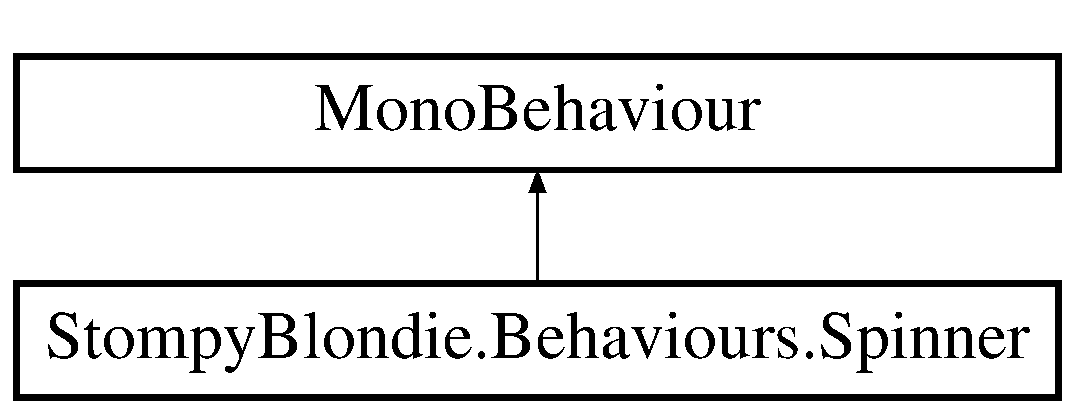
\includegraphics[height=2.000000cm]{class_stompy_blondie_1_1_behaviours_1_1_spinner}
\end{center}
\end{figure}
\subsection*{Public Member Functions}
\begin{DoxyCompactItemize}
\item 
void \mbox{\hyperlink{class_stompy_blondie_1_1_behaviours_1_1_spinner_a33ccb86c5abbeec77a4039cf8be1dd64}{Update}} ()
\end{DoxyCompactItemize}
\subsection*{Public Attributes}
\begin{DoxyCompactItemize}
\item 
\mbox{\hyperlink{namespace_stompy_blondie_1_1_common_1_1_types_aa8d41922aaa5f468ef8e2c8f8e083084}{Rotational\+Direction}} \mbox{\hyperlink{class_stompy_blondie_1_1_behaviours_1_1_spinner_a8443ae6a767b91a6d398416f08fe69be}{direction}}
\item 
float \mbox{\hyperlink{class_stompy_blondie_1_1_behaviours_1_1_spinner_a34128a5d487db9bf69d6e9aa84ec2130}{speed}} = 50f
\end{DoxyCompactItemize}


\subsection{Member Function Documentation}
\mbox{\Hypertarget{class_stompy_blondie_1_1_behaviours_1_1_spinner_a33ccb86c5abbeec77a4039cf8be1dd64}\label{class_stompy_blondie_1_1_behaviours_1_1_spinner_a33ccb86c5abbeec77a4039cf8be1dd64}} 
\index{Stompy\+Blondie\+::\+Behaviours\+::\+Spinner@{Stompy\+Blondie\+::\+Behaviours\+::\+Spinner}!Update@{Update}}
\index{Update@{Update}!Stompy\+Blondie\+::\+Behaviours\+::\+Spinner@{Stompy\+Blondie\+::\+Behaviours\+::\+Spinner}}
\subsubsection{\texorpdfstring{Update()}{Update()}}
{\footnotesize\ttfamily void Stompy\+Blondie.\+Behaviours.\+Spinner.\+Update (\begin{DoxyParamCaption}{ }\end{DoxyParamCaption})\hspace{0.3cm}{\ttfamily [inline]}}



\subsection{Member Data Documentation}
\mbox{\Hypertarget{class_stompy_blondie_1_1_behaviours_1_1_spinner_a8443ae6a767b91a6d398416f08fe69be}\label{class_stompy_blondie_1_1_behaviours_1_1_spinner_a8443ae6a767b91a6d398416f08fe69be}} 
\index{Stompy\+Blondie\+::\+Behaviours\+::\+Spinner@{Stompy\+Blondie\+::\+Behaviours\+::\+Spinner}!direction@{direction}}
\index{direction@{direction}!Stompy\+Blondie\+::\+Behaviours\+::\+Spinner@{Stompy\+Blondie\+::\+Behaviours\+::\+Spinner}}
\subsubsection{\texorpdfstring{direction}{direction}}
{\footnotesize\ttfamily \mbox{\hyperlink{namespace_stompy_blondie_1_1_common_1_1_types_aa8d41922aaa5f468ef8e2c8f8e083084}{Rotational\+Direction}} Stompy\+Blondie.\+Behaviours.\+Spinner.\+direction}

\mbox{\Hypertarget{class_stompy_blondie_1_1_behaviours_1_1_spinner_a34128a5d487db9bf69d6e9aa84ec2130}\label{class_stompy_blondie_1_1_behaviours_1_1_spinner_a34128a5d487db9bf69d6e9aa84ec2130}} 
\index{Stompy\+Blondie\+::\+Behaviours\+::\+Spinner@{Stompy\+Blondie\+::\+Behaviours\+::\+Spinner}!speed@{speed}}
\index{speed@{speed}!Stompy\+Blondie\+::\+Behaviours\+::\+Spinner@{Stompy\+Blondie\+::\+Behaviours\+::\+Spinner}}
\subsubsection{\texorpdfstring{speed}{speed}}
{\footnotesize\ttfamily float Stompy\+Blondie.\+Behaviours.\+Spinner.\+speed = 50f}



The documentation for this class was generated from the following file\+:\begin{DoxyCompactItemize}
\item 
Behaviours/\mbox{\hyperlink{_spinner_8cs}{Spinner.\+cs}}\end{DoxyCompactItemize}

\hypertarget{class_stompy_blondie_1_1_a_i_1_1_tilemap_navigation}{}\section{Stompy\+Blondie.\+A\+I.\+Tilemap\+Navigation Class Reference}
\label{class_stompy_blondie_1_1_a_i_1_1_tilemap_navigation}\index{Stompy\+Blondie.\+A\+I.\+Tilemap\+Navigation@{Stompy\+Blondie.\+A\+I.\+Tilemap\+Navigation}}


The documentation for this class was generated from the following file\+:\begin{DoxyCompactItemize}
\item 
A\+I/Tilemap\+Navigation.\+cs\end{DoxyCompactItemize}

\hypertarget{class_stompy_blondie_1_1_utils_1_1_time_lerp}{}\section{Stompy\+Blondie.\+Utils.\+Time\+Lerp Class Reference}
\label{class_stompy_blondie_1_1_utils_1_1_time_lerp}\index{Stompy\+Blondie.\+Utils.\+Time\+Lerp@{Stompy\+Blondie.\+Utils.\+Time\+Lerp}}
Inheritance diagram for Stompy\+Blondie.\+Utils.\+Time\+Lerp\+:\begin{figure}[H]
\begin{center}
\leavevmode
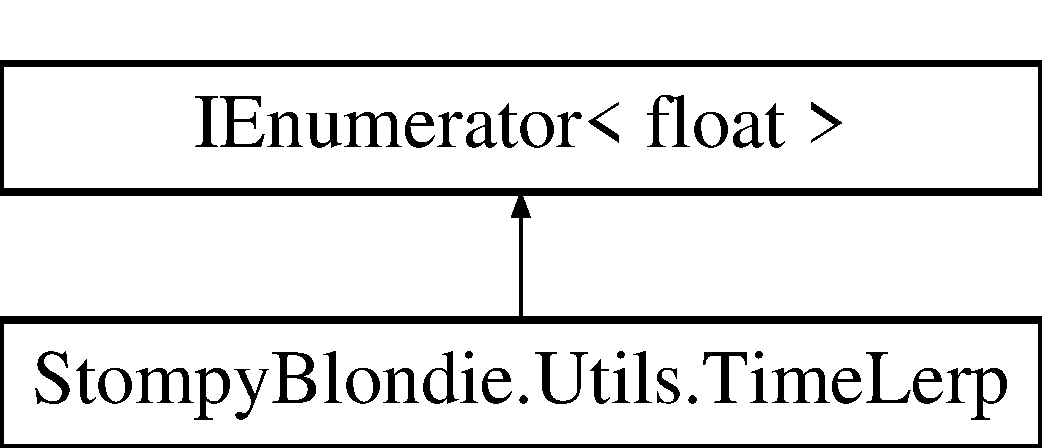
\includegraphics[height=2.000000cm]{class_stompy_blondie_1_1_utils_1_1_time_lerp}
\end{center}
\end{figure}
\subsection*{Public Member Functions}
\begin{DoxyCompactItemize}
\item 
\mbox{\Hypertarget{class_stompy_blondie_1_1_utils_1_1_time_lerp_a29f7e8faa0c774f1be10d5d75f021abb}\label{class_stompy_blondie_1_1_utils_1_1_time_lerp_a29f7e8faa0c774f1be10d5d75f021abb}} 
{\bfseries Time\+Lerp} (float duration\+Seconds)
\item 
\mbox{\Hypertarget{class_stompy_blondie_1_1_utils_1_1_time_lerp_a2919d12fff90522ccbe3d24ade54c6b8}\label{class_stompy_blondie_1_1_utils_1_1_time_lerp_a2919d12fff90522ccbe3d24ade54c6b8}} 
bool {\bfseries Move\+Next} ()
\item 
\mbox{\Hypertarget{class_stompy_blondie_1_1_utils_1_1_time_lerp_a471266f48a72cf51013cc9333b026076}\label{class_stompy_blondie_1_1_utils_1_1_time_lerp_a471266f48a72cf51013cc9333b026076}} 
void {\bfseries Reset} ()
\item 
\mbox{\Hypertarget{class_stompy_blondie_1_1_utils_1_1_time_lerp_a927abfb7ac2193812d8ffb4d557dec3c}\label{class_stompy_blondie_1_1_utils_1_1_time_lerp_a927abfb7ac2193812d8ffb4d557dec3c}} 
void {\bfseries Dispose} ()
\end{DoxyCompactItemize}
\subsection*{Properties}
\begin{DoxyCompactItemize}
\item 
\mbox{\Hypertarget{class_stompy_blondie_1_1_utils_1_1_time_lerp_a1caee886c2d6305e949dfa241553432f}\label{class_stompy_blondie_1_1_utils_1_1_time_lerp_a1caee886c2d6305e949dfa241553432f}} 
float {\bfseries Current}\hspace{0.3cm}{\ttfamily  \mbox{[}get\mbox{]}}
\end{DoxyCompactItemize}


The documentation for this class was generated from the following file\+:\begin{DoxyCompactItemize}
\item 
Utils/Lerp\+Helper.\+cs\end{DoxyCompactItemize}

\hypertarget{class_stompy_blondie_1_1_utils_1_1_time_lerper}{}\section{Stompy\+Blondie.\+Utils.\+Time\+Lerper Class Reference}
\label{class_stompy_blondie_1_1_utils_1_1_time_lerper}\index{Stompy\+Blondie.\+Utils.\+Time\+Lerper@{Stompy\+Blondie.\+Utils.\+Time\+Lerper}}
Inheritance diagram for Stompy\+Blondie.\+Utils.\+Time\+Lerper\+:\begin{figure}[H]
\begin{center}
\leavevmode
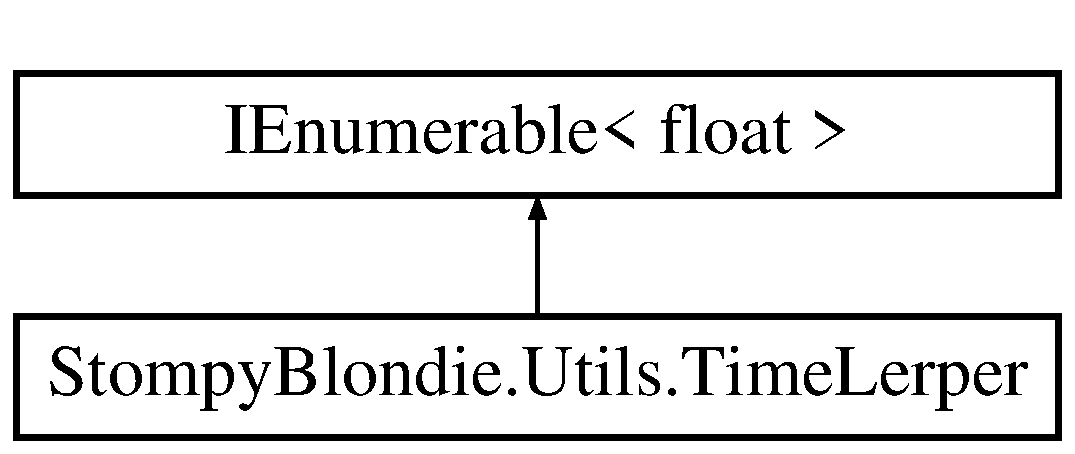
\includegraphics[height=2.000000cm]{class_stompy_blondie_1_1_utils_1_1_time_lerper}
\end{center}
\end{figure}
\subsection*{Public Member Functions}
\begin{DoxyCompactItemize}
\item 
\mbox{\hyperlink{class_stompy_blondie_1_1_utils_1_1_time_lerper_a921b38718ec7717d1aa4ba43e932a067}{Time\+Lerper}} (float duration\+Seconds)
\item 
I\+Enumerator$<$ float $>$ \mbox{\hyperlink{class_stompy_blondie_1_1_utils_1_1_time_lerper_a94f254b4f590804aaa2acbb2f6fb51c9}{Get\+Enumerator}} ()
\end{DoxyCompactItemize}


\subsection{Constructor \& Destructor Documentation}
\mbox{\Hypertarget{class_stompy_blondie_1_1_utils_1_1_time_lerper_a921b38718ec7717d1aa4ba43e932a067}\label{class_stompy_blondie_1_1_utils_1_1_time_lerper_a921b38718ec7717d1aa4ba43e932a067}} 
\index{Stompy\+Blondie\+::\+Utils\+::\+Time\+Lerper@{Stompy\+Blondie\+::\+Utils\+::\+Time\+Lerper}!Time\+Lerper@{Time\+Lerper}}
\index{Time\+Lerper@{Time\+Lerper}!Stompy\+Blondie\+::\+Utils\+::\+Time\+Lerper@{Stompy\+Blondie\+::\+Utils\+::\+Time\+Lerper}}
\subsubsection{\texorpdfstring{Time\+Lerper()}{TimeLerper()}}
{\footnotesize\ttfamily Stompy\+Blondie.\+Utils.\+Time\+Lerper.\+Time\+Lerper (\begin{DoxyParamCaption}\item[{float}]{duration\+Seconds }\end{DoxyParamCaption})\hspace{0.3cm}{\ttfamily [inline]}}



\subsection{Member Function Documentation}
\mbox{\Hypertarget{class_stompy_blondie_1_1_utils_1_1_time_lerper_a94f254b4f590804aaa2acbb2f6fb51c9}\label{class_stompy_blondie_1_1_utils_1_1_time_lerper_a94f254b4f590804aaa2acbb2f6fb51c9}} 
\index{Stompy\+Blondie\+::\+Utils\+::\+Time\+Lerper@{Stompy\+Blondie\+::\+Utils\+::\+Time\+Lerper}!Get\+Enumerator@{Get\+Enumerator}}
\index{Get\+Enumerator@{Get\+Enumerator}!Stompy\+Blondie\+::\+Utils\+::\+Time\+Lerper@{Stompy\+Blondie\+::\+Utils\+::\+Time\+Lerper}}
\subsubsection{\texorpdfstring{Get\+Enumerator()}{GetEnumerator()}}
{\footnotesize\ttfamily I\+Enumerator$<$float$>$ Stompy\+Blondie.\+Utils.\+Time\+Lerper.\+Get\+Enumerator (\begin{DoxyParamCaption}{ }\end{DoxyParamCaption})\hspace{0.3cm}{\ttfamily [inline]}}



The documentation for this class was generated from the following file\+:\begin{DoxyCompactItemize}
\item 
Utils/\mbox{\hyperlink{_lerp_helper_8cs}{Lerp\+Helper.\+cs}}\end{DoxyCompactItemize}

\chapter{File Documentation}
\hypertarget{_navigation_map_debug_renderer_8cs}{}\section{A\+I/\+Navigation\+Map\+Debug\+Renderer.cs File Reference}
\label{_navigation_map_debug_renderer_8cs}\index{A\+I/\+Navigation\+Map\+Debug\+Renderer.\+cs@{A\+I/\+Navigation\+Map\+Debug\+Renderer.\+cs}}
\subsection*{Classes}
\begin{DoxyCompactItemize}
\item 
class \mbox{\hyperlink{class_stompy_blondie_1_1_a_i_1_1_navigation_map_debug_renderer}{Stompy\+Blondie.\+A\+I.\+Navigation\+Map\+Debug\+Renderer}}
\end{DoxyCompactItemize}
\subsection*{Namespaces}
\begin{DoxyCompactItemize}
\item 
namespace \mbox{\hyperlink{namespace_stompy_blondie_1_1_a_i}{Stompy\+Blondie.\+AI}}
\end{DoxyCompactItemize}

\hypertarget{_tilemap_navigation_8cs}{}\section{A\+I/\+Tilemap\+Navigation.cs File Reference}
\label{_tilemap_navigation_8cs}\index{A\+I/\+Tilemap\+Navigation.\+cs@{A\+I/\+Tilemap\+Navigation.\+cs}}
\subsection*{Classes}
\begin{DoxyCompactItemize}
\item 
struct \mbox{\hyperlink{struct_stompy_blondie_1_1_a_i_1_1_navigation_point_link}{Stompy\+Blondie.\+A\+I.\+Navigation\+Point\+Link}}
\item 
struct \mbox{\hyperlink{struct_stompy_blondie_1_1_a_i_1_1_navigation_point}{Stompy\+Blondie.\+A\+I.\+Navigation\+Point}}
\item 
class \mbox{\hyperlink{class_stompy_blondie_1_1_a_i_1_1_navigation_map}{Stompy\+Blondie.\+A\+I.\+Navigation\+Map}}
\item 
class \mbox{\hyperlink{class_stompy_blondie_1_1_a_i_1_1_tilemap_navigation}{Stompy\+Blondie.\+A\+I.\+Tilemap\+Navigation}}
\end{DoxyCompactItemize}
\subsection*{Namespaces}
\begin{DoxyCompactItemize}
\item 
namespace \mbox{\hyperlink{namespace_stompy_blondie_1_1_a_i}{Stompy\+Blondie.\+AI}}
\end{DoxyCompactItemize}

\hypertarget{_bobber_8cs}{}\section{Behaviours/\+Bobber.cs File Reference}
\label{_bobber_8cs}\index{Behaviours/\+Bobber.\+cs@{Behaviours/\+Bobber.\+cs}}
\subsection*{Classes}
\begin{DoxyCompactItemize}
\item 
class \mbox{\hyperlink{class_stompy_blondie_1_1_behaviours_1_1_bobber}{Stompy\+Blondie.\+Behaviours.\+Bobber}}
\end{DoxyCompactItemize}
\subsection*{Namespaces}
\begin{DoxyCompactItemize}
\item 
namespace \mbox{\hyperlink{namespace_stompy_blondie_1_1_behaviours}{Stompy\+Blondie.\+Behaviours}}
\end{DoxyCompactItemize}

\hypertarget{_face_camera_8cs}{}\section{Behaviours/\+Face\+Camera.cs File Reference}
\label{_face_camera_8cs}\index{Behaviours/\+Face\+Camera.\+cs@{Behaviours/\+Face\+Camera.\+cs}}
\subsection*{Classes}
\begin{DoxyCompactItemize}
\item 
class \mbox{\hyperlink{class_stompy_blondie_1_1_behaviours_1_1_face_camera}{Stompy\+Blondie.\+Behaviours.\+Face\+Camera}}
\end{DoxyCompactItemize}
\subsection*{Namespaces}
\begin{DoxyCompactItemize}
\item 
namespace \mbox{\hyperlink{namespace_stompy_blondie_1_1_behaviours}{Stompy\+Blondie.\+Behaviours}}
\end{DoxyCompactItemize}

\hypertarget{_is_mouse_over_8cs}{}\section{Behaviours/\+Is\+Mouse\+Over.cs File Reference}
\label{_is_mouse_over_8cs}\index{Behaviours/\+Is\+Mouse\+Over.\+cs@{Behaviours/\+Is\+Mouse\+Over.\+cs}}
\subsection*{Classes}
\begin{DoxyCompactItemize}
\item 
class \mbox{\hyperlink{class_stompy_blondie_1_1_behaviours_1_1_is_mouse_over}{Stompy\+Blondie.\+Behaviours.\+Is\+Mouse\+Over}}
\end{DoxyCompactItemize}
\subsection*{Namespaces}
\begin{DoxyCompactItemize}
\item 
namespace \mbox{\hyperlink{namespace_stompy_blondie_1_1_behaviours}{Stompy\+Blondie.\+Behaviours}}
\end{DoxyCompactItemize}

\hypertarget{_spinner_8cs}{}\section{Behaviours/\+Spinner.cs File Reference}
\label{_spinner_8cs}\index{Behaviours/\+Spinner.\+cs@{Behaviours/\+Spinner.\+cs}}
\subsection*{Classes}
\begin{DoxyCompactItemize}
\item 
class \mbox{\hyperlink{class_stompy_blondie_1_1_behaviours_1_1_spinner}{Stompy\+Blondie.\+Behaviours.\+Spinner}}
\end{DoxyCompactItemize}
\subsection*{Namespaces}
\begin{DoxyCompactItemize}
\item 
namespace \mbox{\hyperlink{namespace_stompy_blondie_1_1_behaviours}{Stompy\+Blondie.\+Behaviours}}
\end{DoxyCompactItemize}

\hypertarget{_ref_8cs}{}\section{Common/\+Ref.cs File Reference}
\label{_ref_8cs}\index{Common/\+Ref.\+cs@{Common/\+Ref.\+cs}}
\subsection*{Classes}
\begin{DoxyCompactItemize}
\item 
class \mbox{\hyperlink{class_stompy_blondie_1_1_common_1_1_ref}{Stompy\+Blondie.\+Common.\+Ref$<$ T $>$}}
\end{DoxyCompactItemize}
\subsection*{Namespaces}
\begin{DoxyCompactItemize}
\item 
namespace \mbox{\hyperlink{namespace_stompy_blondie_1_1_common}{Stompy\+Blondie.\+Common}}
\end{DoxyCompactItemize}

\hypertarget{_types_8cs}{}\section{Common/\+Types.cs File Reference}
\label{_types_8cs}\index{Common/\+Types.\+cs@{Common/\+Types.\+cs}}
\subsection*{Classes}
\begin{DoxyCompactItemize}
\item 
class {\bfseries Stompy\+Blondie.\+Common.\+Types.\+Pos\+Type\+Converter}
\item 
struct \mbox{\hyperlink{struct_stompy_blondie_1_1_common_1_1_types_1_1_pos}{Stompy\+Blondie.\+Common.\+Types.\+Pos}}
\end{DoxyCompactItemize}
\subsection*{Namespaces}
\begin{DoxyCompactItemize}
\item 
namespace \mbox{\hyperlink{namespace_stompy_blondie_1_1_common_1_1_types}{Stompy\+Blondie.\+Common.\+Types}}
\end{DoxyCompactItemize}
\subsection*{Enumerations}
\begin{DoxyCompactItemize}
\item 
enum \mbox{\hyperlink{namespace_stompy_blondie_1_1_common_1_1_types_a2477d455b973b989d248635a56ffbd25}{Stompy\+Blondie.\+Common.\+Types.\+Direction}} \{ \mbox{\hyperlink{namespace_stompy_blondie_1_1_common_1_1_types_a2477d455b973b989d248635a56ffbd25a08a38277b0309070706f6652eeae9a53}{Stompy\+Blondie.\+Common.\+Types.\+Direction.\+Down}}, 
\mbox{\hyperlink{namespace_stompy_blondie_1_1_common_1_1_types_a2477d455b973b989d248635a56ffbd25a945d5e233cf7d6240f6b783b36a374ff}{Stompy\+Blondie.\+Common.\+Types.\+Direction.\+Left}}, 
\mbox{\hyperlink{namespace_stompy_blondie_1_1_common_1_1_types_a2477d455b973b989d248635a56ffbd25a258f49887ef8d14ac268c92b02503aaa}{Stompy\+Blondie.\+Common.\+Types.\+Direction.\+Up}}, 
\mbox{\hyperlink{namespace_stompy_blondie_1_1_common_1_1_types_a2477d455b973b989d248635a56ffbd25a92b09c7c48c520c3c55e497875da437c}{Stompy\+Blondie.\+Common.\+Types.\+Direction.\+Right}}
 \}
\item 
enum \mbox{\hyperlink{namespace_stompy_blondie_1_1_common_1_1_types_a67d21ccf6a23cdea91c271cce76f920f}{Stompy\+Blondie.\+Common.\+Types.\+Eight\+Direction}} \{ \newline
\mbox{\hyperlink{namespace_stompy_blondie_1_1_common_1_1_types_a67d21ccf6a23cdea91c271cce76f920fa08a38277b0309070706f6652eeae9a53}{Stompy\+Blondie.\+Common.\+Types.\+Eight\+Direction.\+Down}}, 
\mbox{\hyperlink{namespace_stompy_blondie_1_1_common_1_1_types_a67d21ccf6a23cdea91c271cce76f920facd7f4772075da1452f8cd3648265b2c1}{Stompy\+Blondie.\+Common.\+Types.\+Eight\+Direction.\+Down\+Left}}, 
\mbox{\hyperlink{namespace_stompy_blondie_1_1_common_1_1_types_a67d21ccf6a23cdea91c271cce76f920fa945d5e233cf7d6240f6b783b36a374ff}{Stompy\+Blondie.\+Common.\+Types.\+Eight\+Direction.\+Left}}, 
\mbox{\hyperlink{namespace_stompy_blondie_1_1_common_1_1_types_a67d21ccf6a23cdea91c271cce76f920fa105736deb2f54f03c011e5f053e08d00}{Stompy\+Blondie.\+Common.\+Types.\+Eight\+Direction.\+Left\+Up}}, 
\newline
\mbox{\hyperlink{namespace_stompy_blondie_1_1_common_1_1_types_a67d21ccf6a23cdea91c271cce76f920fa258f49887ef8d14ac268c92b02503aaa}{Stompy\+Blondie.\+Common.\+Types.\+Eight\+Direction.\+Up}}, 
\mbox{\hyperlink{namespace_stompy_blondie_1_1_common_1_1_types_a67d21ccf6a23cdea91c271cce76f920faee94ab0297ae02df64791255d0a3551e}{Stompy\+Blondie.\+Common.\+Types.\+Eight\+Direction.\+Up\+Right}}, 
\mbox{\hyperlink{namespace_stompy_blondie_1_1_common_1_1_types_a67d21ccf6a23cdea91c271cce76f920fa92b09c7c48c520c3c55e497875da437c}{Stompy\+Blondie.\+Common.\+Types.\+Eight\+Direction.\+Right}}, 
\mbox{\hyperlink{namespace_stompy_blondie_1_1_common_1_1_types_a67d21ccf6a23cdea91c271cce76f920fac7ff24224bc4b699e06c58a663ac618c}{Stompy\+Blondie.\+Common.\+Types.\+Eight\+Direction.\+Right\+Down}}
 \}
\item 
enum \mbox{\hyperlink{namespace_stompy_blondie_1_1_common_1_1_types_aa8d41922aaa5f468ef8e2c8f8e083084}{Stompy\+Blondie.\+Common.\+Types.\+Rotational\+Direction}} \{ \mbox{\hyperlink{namespace_stompy_blondie_1_1_common_1_1_types_aa8d41922aaa5f468ef8e2c8f8e083084aba360a794737bcc8657a5b6e870d7ba8}{Stompy\+Blondie.\+Common.\+Types.\+Rotational\+Direction.\+Clockwise}}, 
\mbox{\hyperlink{namespace_stompy_blondie_1_1_common_1_1_types_aa8d41922aaa5f468ef8e2c8f8e083084a3ac558edd1e7ab76b05ea7e3eef91b54}{Stompy\+Blondie.\+Common.\+Types.\+Rotational\+Direction.\+Anti\+Clockwise}}
 \}
\end{DoxyCompactItemize}

\hypertarget{_scene_auto_loader_8cs}{}\section{Editor/\+Scene\+Auto\+Loader.cs File Reference}
\label{_scene_auto_loader_8cs}\index{Editor/\+Scene\+Auto\+Loader.\+cs@{Editor/\+Scene\+Auto\+Loader.\+cs}}
\subsection*{Classes}
\begin{DoxyCompactItemize}
\item 
class {\bfseries Scene\+Auto\+Loader}
\begin{DoxyCompactList}\small\item\em Scene auto loader. \end{DoxyCompactList}\end{DoxyCompactItemize}

\hypertarget{_extension_audio_source_8cs}{}\section{Extensions/\+Extension\+Audio\+Source.cs File Reference}
\label{_extension_audio_source_8cs}\index{Extensions/\+Extension\+Audio\+Source.\+cs@{Extensions/\+Extension\+Audio\+Source.\+cs}}
\subsection*{Classes}
\begin{DoxyCompactItemize}
\item 
class {\bfseries Stompy\+Blondie.\+Extensions.\+Extension\+Audio\+Source}
\end{DoxyCompactItemize}
\subsection*{Namespaces}
\begin{DoxyCompactItemize}
\item 
namespace \mbox{\hyperlink{namespace_stompy_blondie_1_1_extensions}{Stompy\+Blondie.\+Extensions}}
\end{DoxyCompactItemize}

\hypertarget{_extension_mono_behaviour_8cs}{}\section{Extensions/\+Extension\+Mono\+Behaviour.cs File Reference}
\label{_extension_mono_behaviour_8cs}\index{Extensions/\+Extension\+Mono\+Behaviour.\+cs@{Extensions/\+Extension\+Mono\+Behaviour.\+cs}}
\subsection*{Classes}
\begin{DoxyCompactItemize}
\item 
class \mbox{\hyperlink{class_stompy_blondie_1_1_extensions_1_1_extension_mono_behaviour}{Stompy\+Blondie.\+Extensions.\+Extension\+Mono\+Behaviour}}
\end{DoxyCompactItemize}
\subsection*{Namespaces}
\begin{DoxyCompactItemize}
\item 
namespace \mbox{\hyperlink{namespace_stompy_blondie_1_1_extensions}{Stompy\+Blondie.\+Extensions}}
\end{DoxyCompactItemize}

\hypertarget{_extension_unity_vector3_8cs}{}\section{Extensions/\+Extension\+Unity\+Vector3.cs File Reference}
\label{_extension_unity_vector3_8cs}\index{Extensions/\+Extension\+Unity\+Vector3.\+cs@{Extensions/\+Extension\+Unity\+Vector3.\+cs}}
\subsection*{Classes}
\begin{DoxyCompactItemize}
\item 
class {\bfseries Stompy\+Blondie.\+Extensions.\+Extension\+Unity\+Vector3}
\end{DoxyCompactItemize}
\subsection*{Namespaces}
\begin{DoxyCompactItemize}
\item 
namespace \mbox{\hyperlink{namespace_stompy_blondie_1_1_extensions}{Stompy\+Blondie.\+Extensions}}
\end{DoxyCompactItemize}

\hypertarget{_a_star_8cs}{}\section{Math/\+A\+Star.cs File Reference}
\label{_a_star_8cs}\index{Math/\+A\+Star.\+cs@{Math/\+A\+Star.\+cs}}
\subsection*{Classes}
\begin{DoxyCompactItemize}
\item 
class \mbox{\hyperlink{class_stompy_blondie_1_1_math_1_1_a_star_node}{Stompy\+Blondie.\+Math.\+A\+Star\+Node}}
\item 
class \mbox{\hyperlink{class_stompy_blondie_1_1_math_1_1_a_star}{Stompy\+Blondie.\+Math.\+A\+Star}}
\end{DoxyCompactItemize}
\subsection*{Namespaces}
\begin{DoxyCompactItemize}
\item 
namespace \mbox{\hyperlink{namespace_stompy_blondie_1_1_math}{Stompy\+Blondie.\+Math}}
\end{DoxyCompactItemize}

\hypertarget{_r_e_a_d_m_e_8md}{}\section{R\+E\+A\+D\+M\+E.\+md File Reference}
\label{_r_e_a_d_m_e_8md}\index{R\+E\+A\+D\+M\+E.\+md@{R\+E\+A\+D\+M\+E.\+md}}

\hypertarget{_effects_manager_8cs}{}\section{Systems/\+Effects\+Manager.cs File Reference}
\label{_effects_manager_8cs}\index{Systems/\+Effects\+Manager.\+cs@{Systems/\+Effects\+Manager.\+cs}}
\subsection*{Classes}
\begin{DoxyCompactItemize}
\item 
class \mbox{\hyperlink{class_stompy_blondie_1_1_systems_1_1_effect}{Stompy\+Blondie.\+Systems.\+Effect}}
\item 
class \mbox{\hyperlink{class_stompy_blondie_1_1_systems_1_1_effects_manager}{Stompy\+Blondie.\+Systems.\+Effects\+Manager}}
\end{DoxyCompactItemize}
\subsection*{Namespaces}
\begin{DoxyCompactItemize}
\item 
namespace \mbox{\hyperlink{namespace_stompy_blondie_1_1_systems}{Stompy\+Blondie.\+Systems}}
\end{DoxyCompactItemize}

\hypertarget{_a_star_8spec_8cs}{}\section{Tests/\+A\+Star.spec.\+cs File Reference}
\label{_a_star_8spec_8cs}\index{Tests/\+A\+Star.\+spec.\+cs@{Tests/\+A\+Star.\+spec.\+cs}}
\subsection*{Classes}
\begin{DoxyCompactItemize}
\item 
class \mbox{\hyperlink{class_stompy_blondie_1_1_tests_1_1_a_star_test}{Stompy\+Blondie.\+Tests.\+A\+Star\+Test}}
\end{DoxyCompactItemize}
\subsection*{Namespaces}
\begin{DoxyCompactItemize}
\item 
namespace \mbox{\hyperlink{namespace_stompy_blondie_1_1_tests}{Stompy\+Blondie.\+Tests}}
\end{DoxyCompactItemize}

\hypertarget{_bone_clone_8cs}{}\section{Utils/\+Bone\+Clone.cs File Reference}
\label{_bone_clone_8cs}\index{Utils/\+Bone\+Clone.\+cs@{Utils/\+Bone\+Clone.\+cs}}
\subsection*{Classes}
\begin{DoxyCompactItemize}
\item 
class \mbox{\hyperlink{class_stompy_blondie_1_1_utils_1_1_bone_clone}{Stompy\+Blondie.\+Utils.\+Bone\+Clone}}
\end{DoxyCompactItemize}
\subsection*{Namespaces}
\begin{DoxyCompactItemize}
\item 
namespace \mbox{\hyperlink{namespace_stompy_blondie_1_1_utils}{Stompy\+Blondie.\+Utils}}
\end{DoxyCompactItemize}

\hypertarget{_direction_helper_8cs}{}\section{Utils/\+Direction\+Helper.cs File Reference}
\label{_direction_helper_8cs}\index{Utils/\+Direction\+Helper.\+cs@{Utils/\+Direction\+Helper.\+cs}}
\subsection*{Classes}
\begin{DoxyCompactItemize}
\item 
class {\bfseries Stompy\+Blondie.\+Utils.\+Direction\+Helper}
\end{DoxyCompactItemize}
\subsection*{Namespaces}
\begin{DoxyCompactItemize}
\item 
namespace \mbox{\hyperlink{namespace_stompy_blondie_1_1_utils}{Stompy\+Blondie.\+Utils}}
\end{DoxyCompactItemize}

\hypertarget{_extension_transform_8cs}{}\section{Utils/\+Extension\+Transform.cs File Reference}
\label{_extension_transform_8cs}\index{Utils/\+Extension\+Transform.\+cs@{Utils/\+Extension\+Transform.\+cs}}
\subsection*{Classes}
\begin{DoxyCompactItemize}
\item 
class {\bfseries Stompy\+Blondie.\+Extensions.\+Extension\+Transform}
\end{DoxyCompactItemize}
\subsection*{Namespaces}
\begin{DoxyCompactItemize}
\item 
namespace \mbox{\hyperlink{namespace_stompy_blondie_1_1_extensions}{Stompy\+Blondie.\+Extensions}}
\end{DoxyCompactItemize}

\hypertarget{_lerp_helper_8cs}{}\section{Utils/\+Lerp\+Helper.cs File Reference}
\label{_lerp_helper_8cs}\index{Utils/\+Lerp\+Helper.\+cs@{Utils/\+Lerp\+Helper.\+cs}}
\subsection*{Classes}
\begin{DoxyCompactItemize}
\item 
class {\bfseries Stompy\+Blondie.\+Utils.\+Lerp\+Helper}
\item 
class \mbox{\hyperlink{class_stompy_blondie_1_1_utils_1_1_time_lerper}{Stompy\+Blondie.\+Utils.\+Time\+Lerper}}
\item 
class \mbox{\hyperlink{class_stompy_blondie_1_1_utils_1_1_time_lerp}{Stompy\+Blondie.\+Utils.\+Time\+Lerp}}
\end{DoxyCompactItemize}
\subsection*{Namespaces}
\begin{DoxyCompactItemize}
\item 
namespace \mbox{\hyperlink{namespace_stompy_blondie_1_1_utils}{Stompy\+Blondie.\+Utils}}
\end{DoxyCompactItemize}

\hypertarget{_scrollbar_helper_8cs}{}\section{Utils/\+Scrollbar\+Helper.cs File Reference}
\label{_scrollbar_helper_8cs}\index{Utils/\+Scrollbar\+Helper.\+cs@{Utils/\+Scrollbar\+Helper.\+cs}}
\subsection*{Classes}
\begin{DoxyCompactItemize}
\item 
class {\bfseries Stompy\+Blondie.\+Utils.\+Scrollbar\+Helper}
\end{DoxyCompactItemize}
\subsection*{Namespaces}
\begin{DoxyCompactItemize}
\item 
namespace \mbox{\hyperlink{namespace_stompy_blondie_1_1_utils}{Stompy\+Blondie.\+Utils}}
\end{DoxyCompactItemize}

%--- End generated contents ---

% Index
\backmatter
\newpage
\phantomsection
\clearemptydoublepage
\addcontentsline{toc}{chapter}{Index}
\printindex

\end{document}
